This chapter dives deep into how Students\&Companies is implemented, integrated and tested.
The chosen approach follows a bottom-up strategy.
It begins with developing and testing foundational elements before integrating the rest of the system.
This gradual process focuses on the independent development of basic modules, which are tested in isolation before being integrated into the larger system.
This independence eliminates the need to consider the entire system upfront, making it easier and faster to address issues and apply changes.
A key factor of this method is the usage of drivers, short tests that simulate the inputs and interactions essential for checking individual modules.

The plan begins with the development and testing of base components, specifically the foundational submanagers within each manager.
Once these base submanagers are implemented and tested, the remaining ones for the same manager are integrated. 
To ensure clarity, when all submanagers of a manager are integrated, they are represented in the diagrams through their respective manager component.

The first step is to implement and test the model.

\begin{figure}[h]
    \centering
    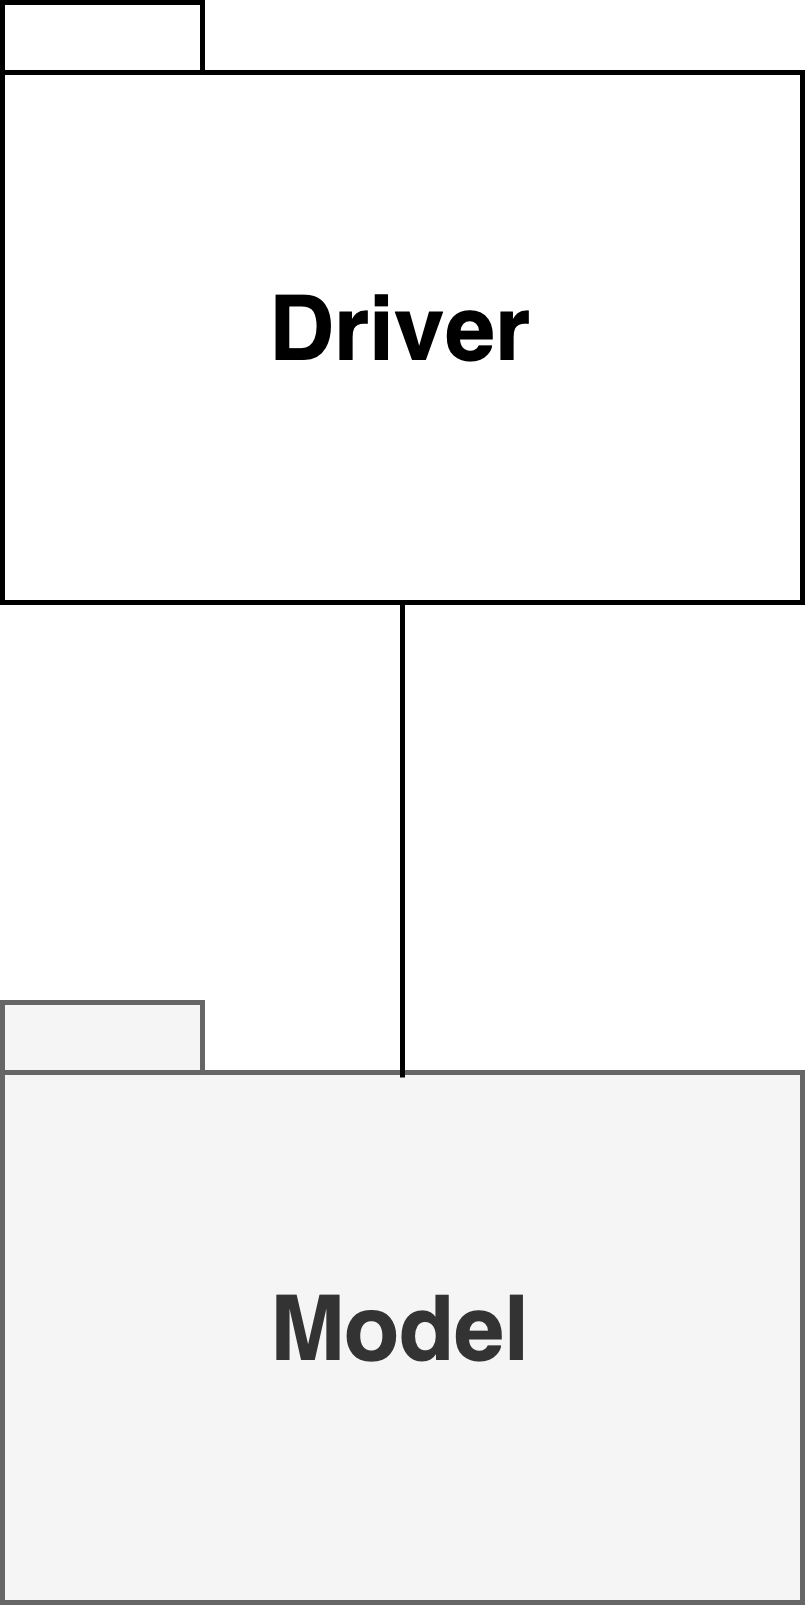
\includegraphics[width=2.5cm]{images/implementation-diagrams/step-1.png}
    \caption{Implementation step 1}
\end{figure}

\newpage
The development proceeds to step two with the user signup and login submanagers.

\begin{figure}[h]
    \centering
    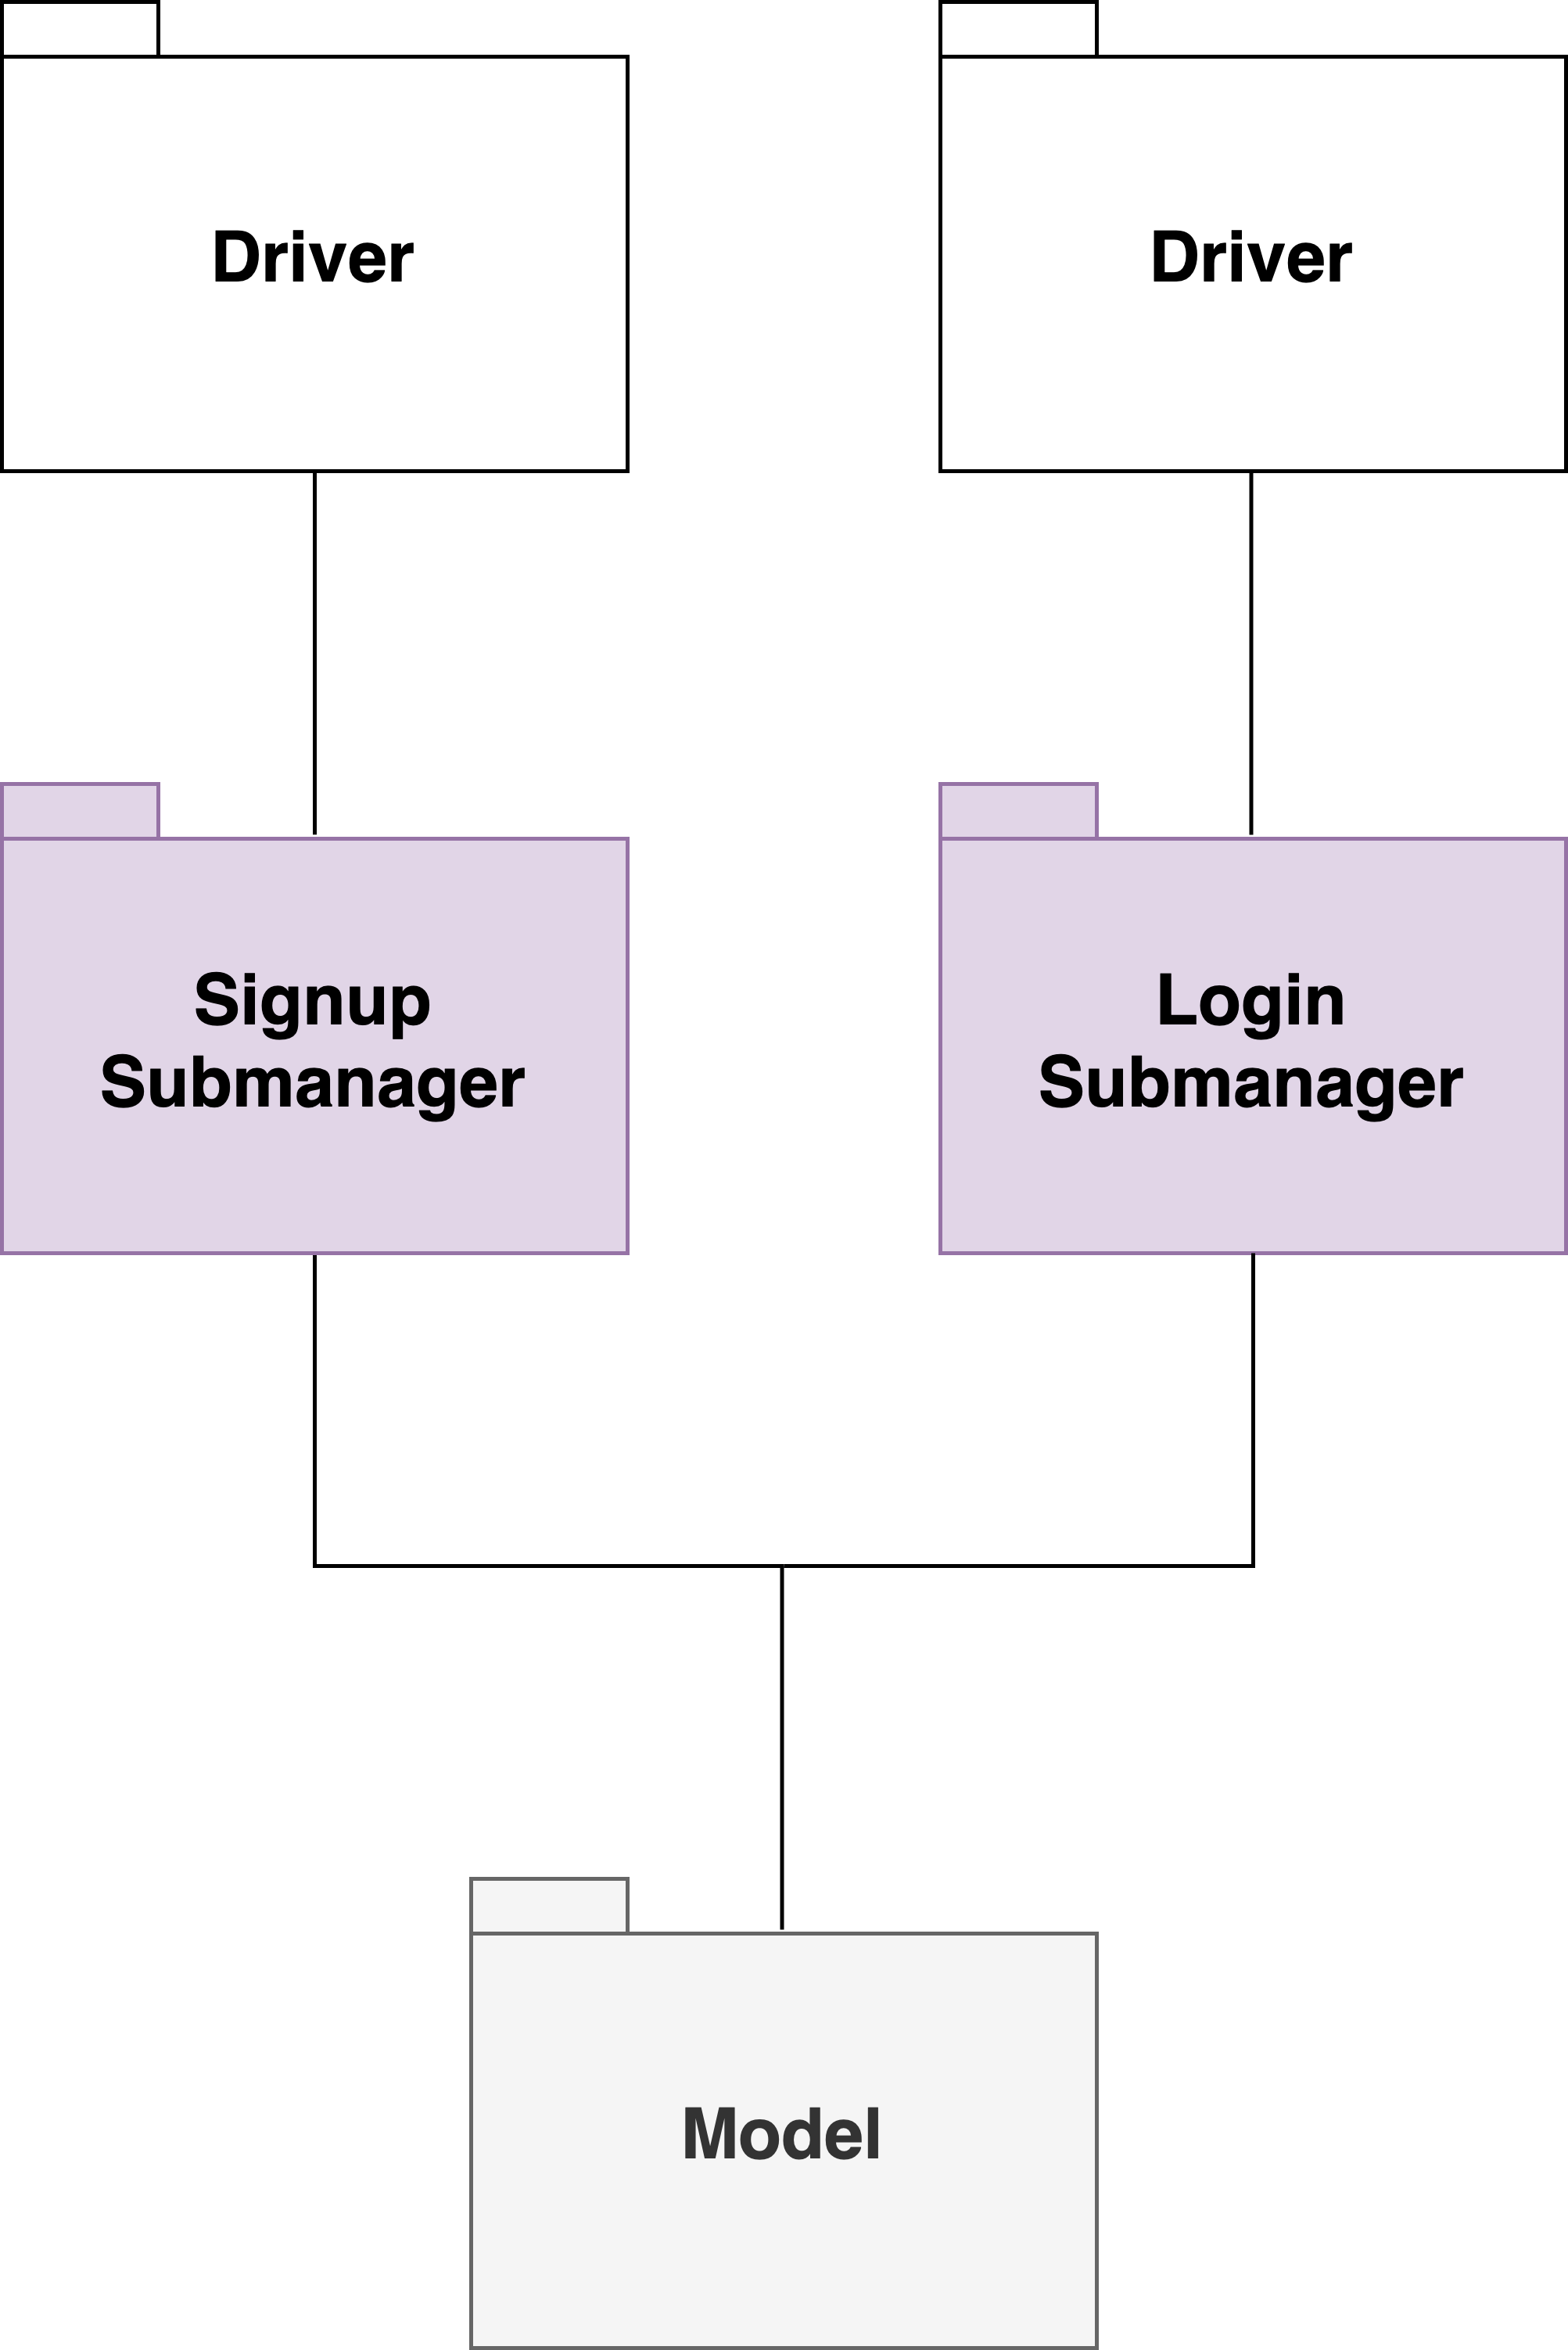
\includegraphics[width=6.5cm]{images/implementation-diagrams/step-2.png}
    \caption{Implementation step 2}
\end{figure}

\newpage
The user management submanager is integrated in the third step.

\begin{figure}[h]
    \centering
    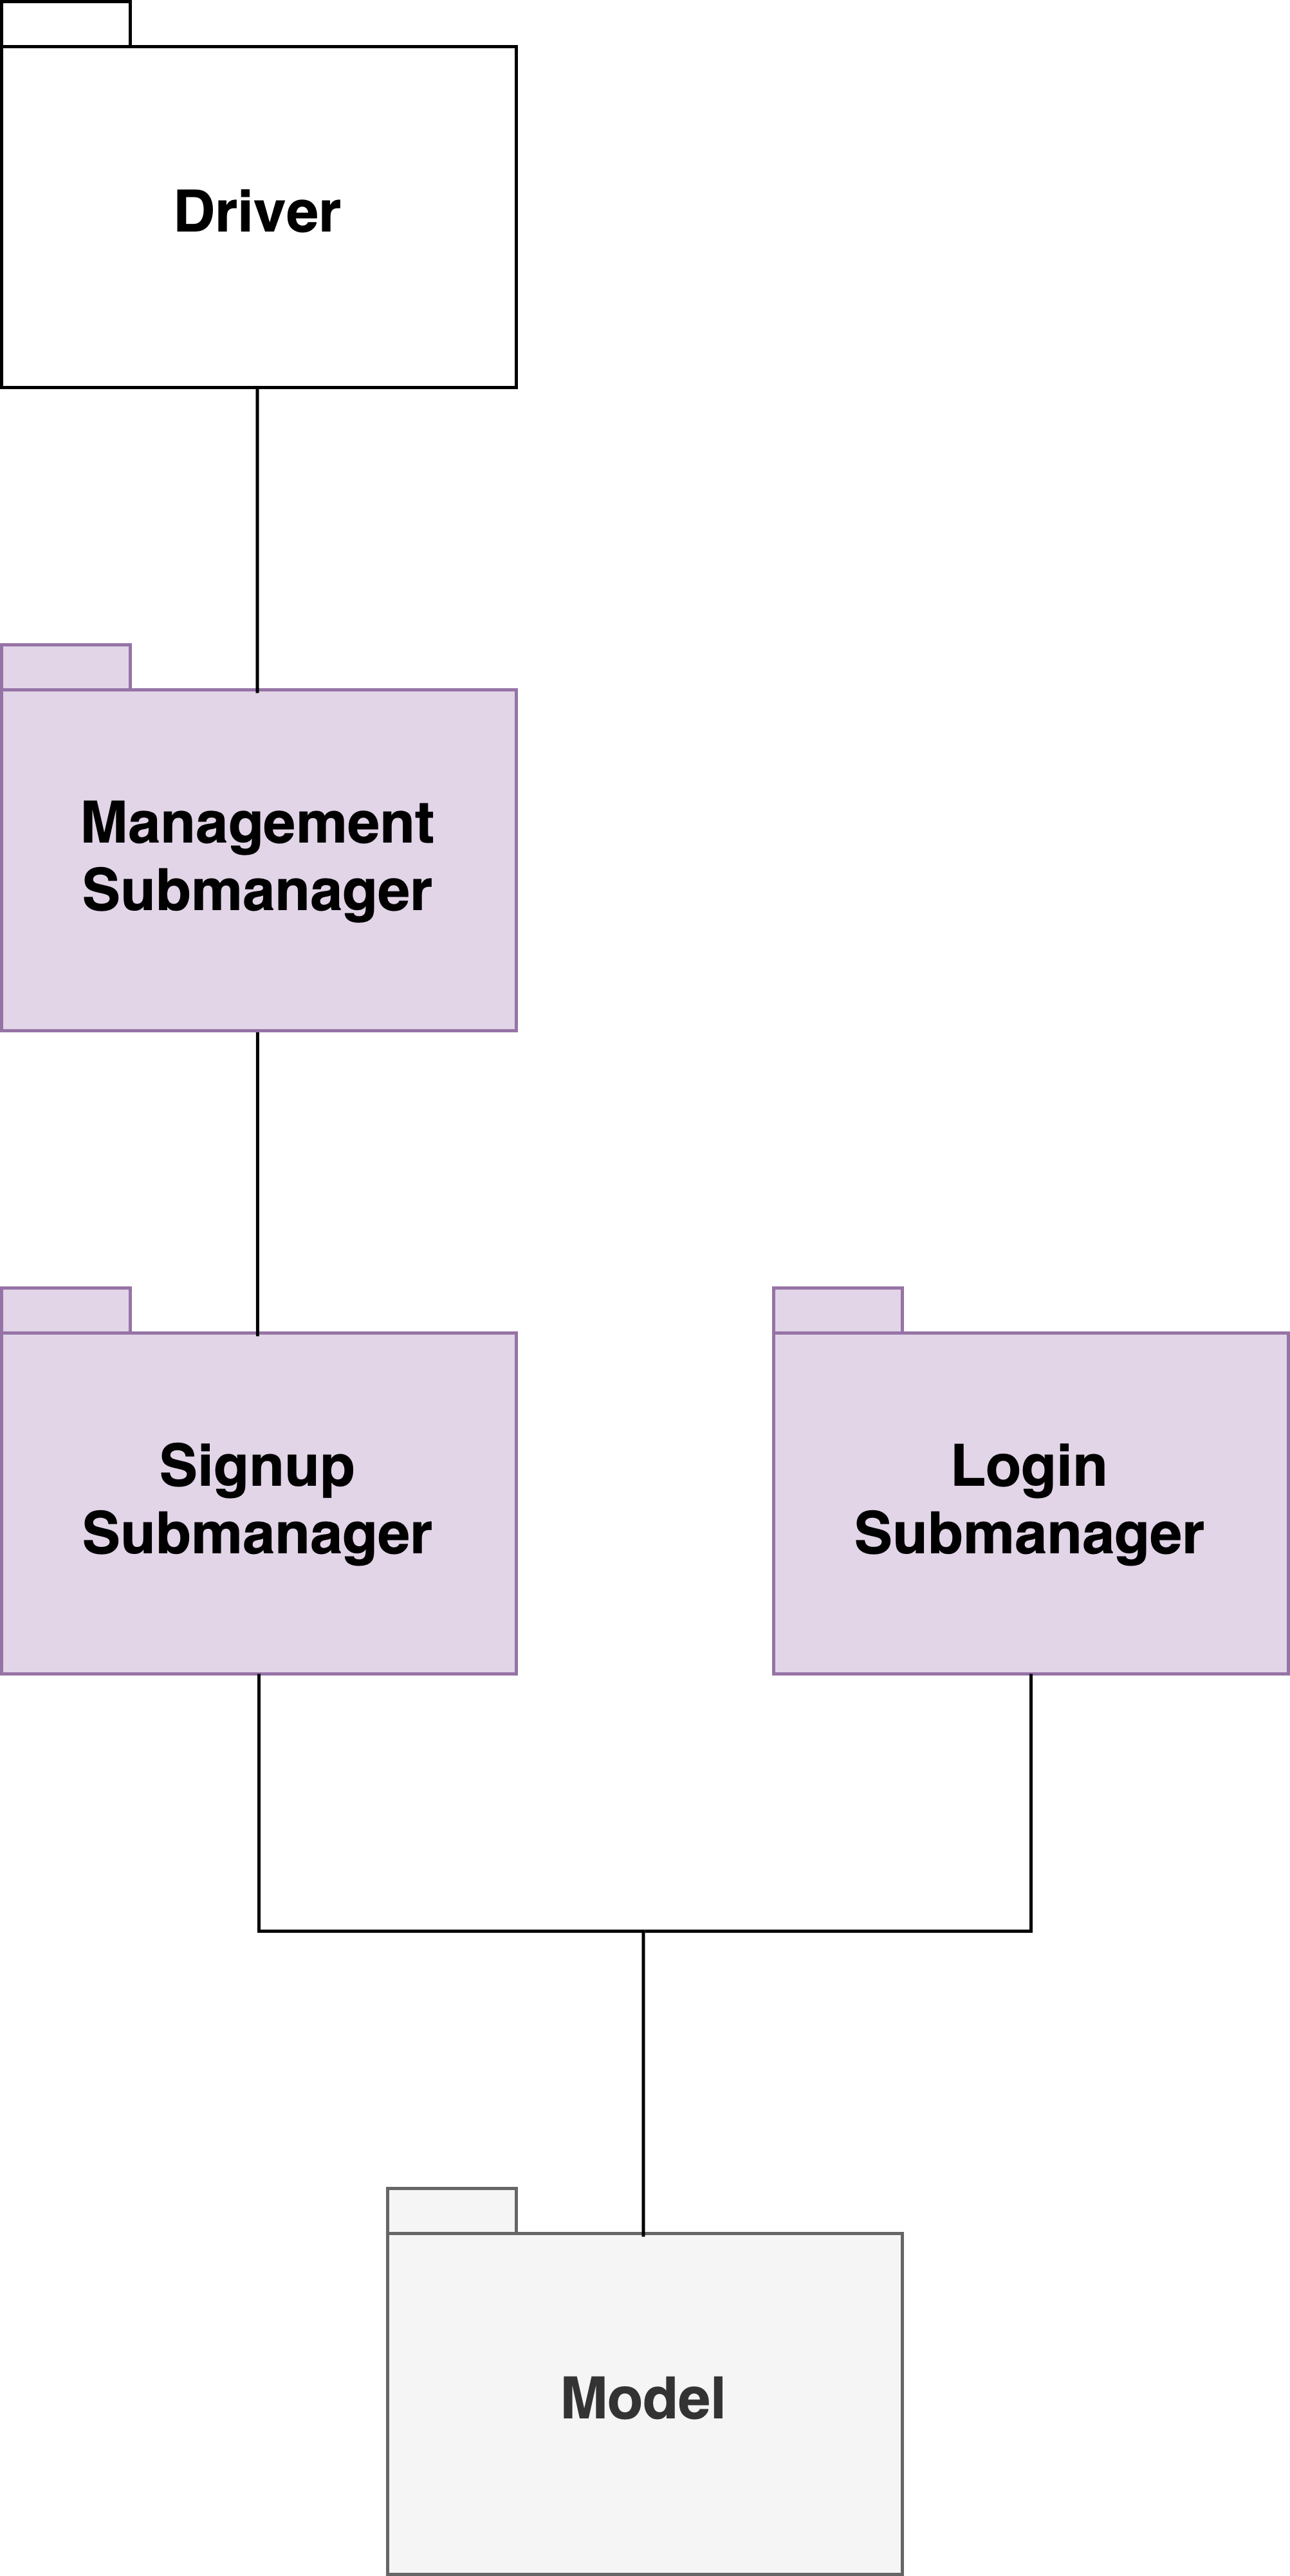
\includegraphics[width=6.5cm]{images/implementation-diagrams/step-3.png}
    \caption{Implementation step 3}
\end{figure}

\newpage
Step four applies the same pattern to the position posting and search submanagers.

\begin{figure}[h]
    \centering
    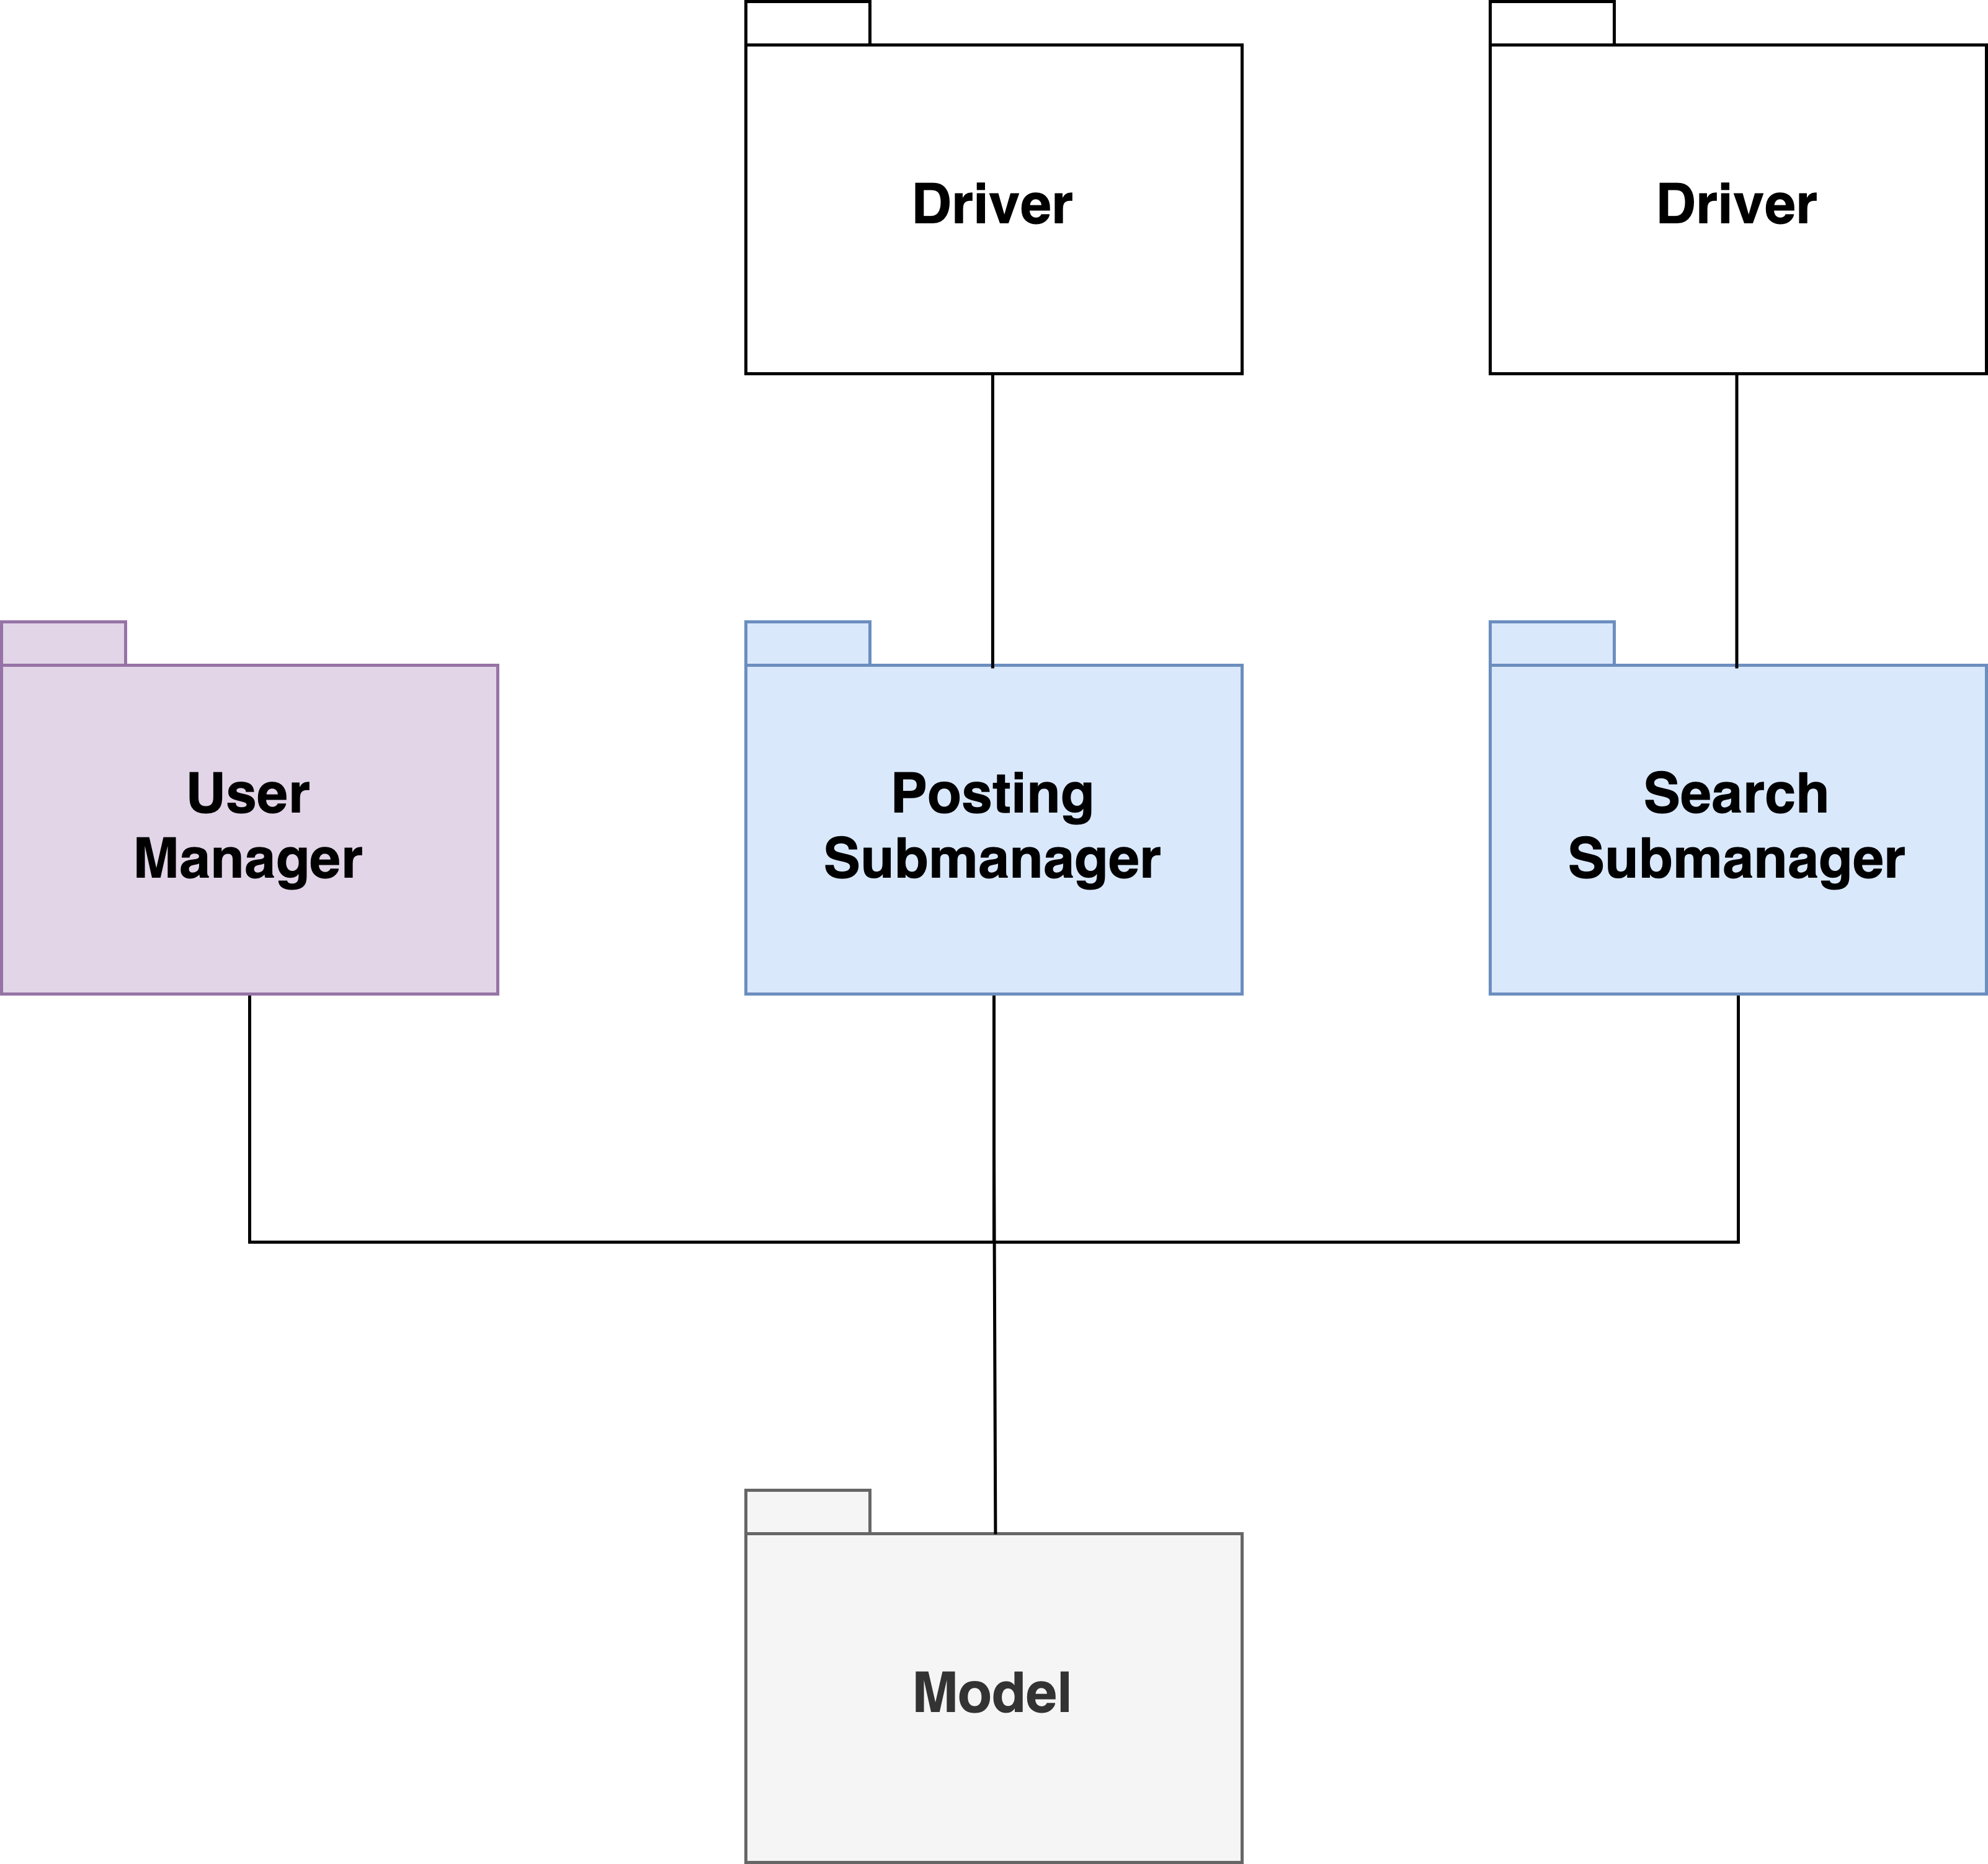
\includegraphics[width=10cm]{images/implementation-diagrams/step-4.png}
    \caption{Implementation step 4}
\end{figure}

\newpage
The position management submanager is integrated in the fifth step.

\begin{figure}[h]
    \centering
    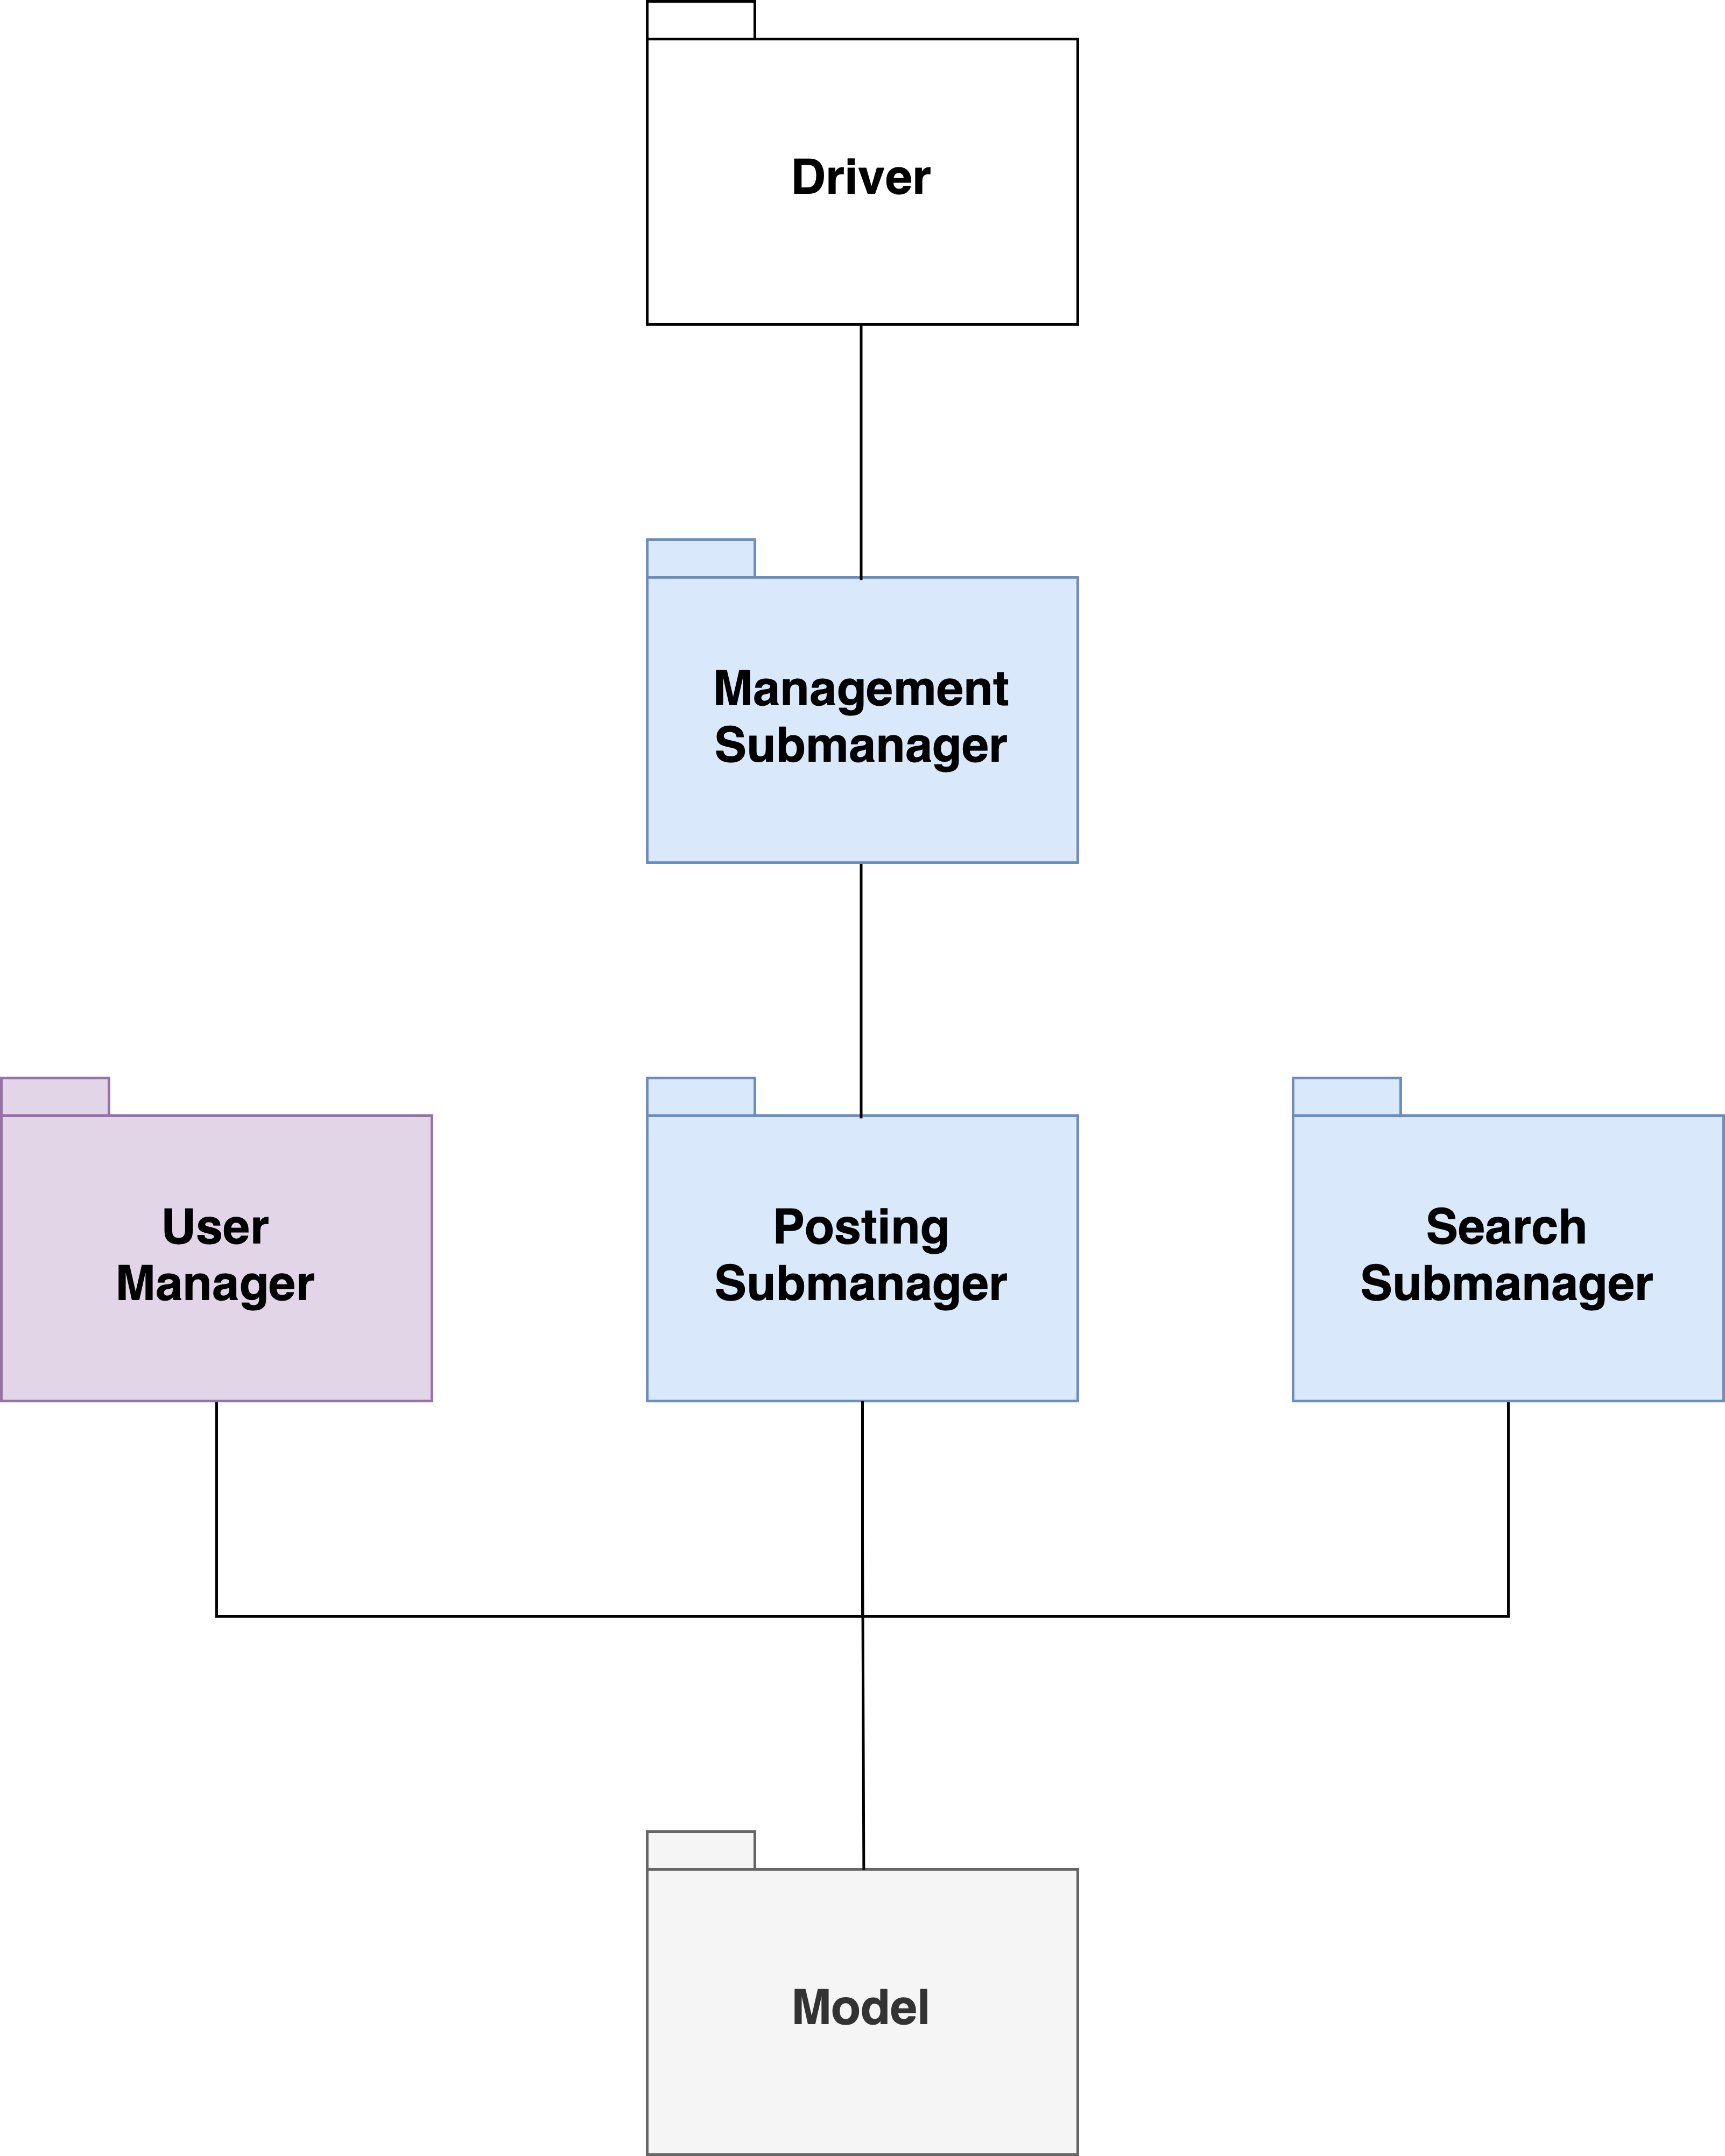
\includegraphics[width=10cm]{images/implementation-diagrams/step-5.png}
    \caption{Implementation step 5}
\end{figure}

\newpage
The development proceeds to step six with the recommendation submanagers.

\begin{figure}[h]
    \centering
    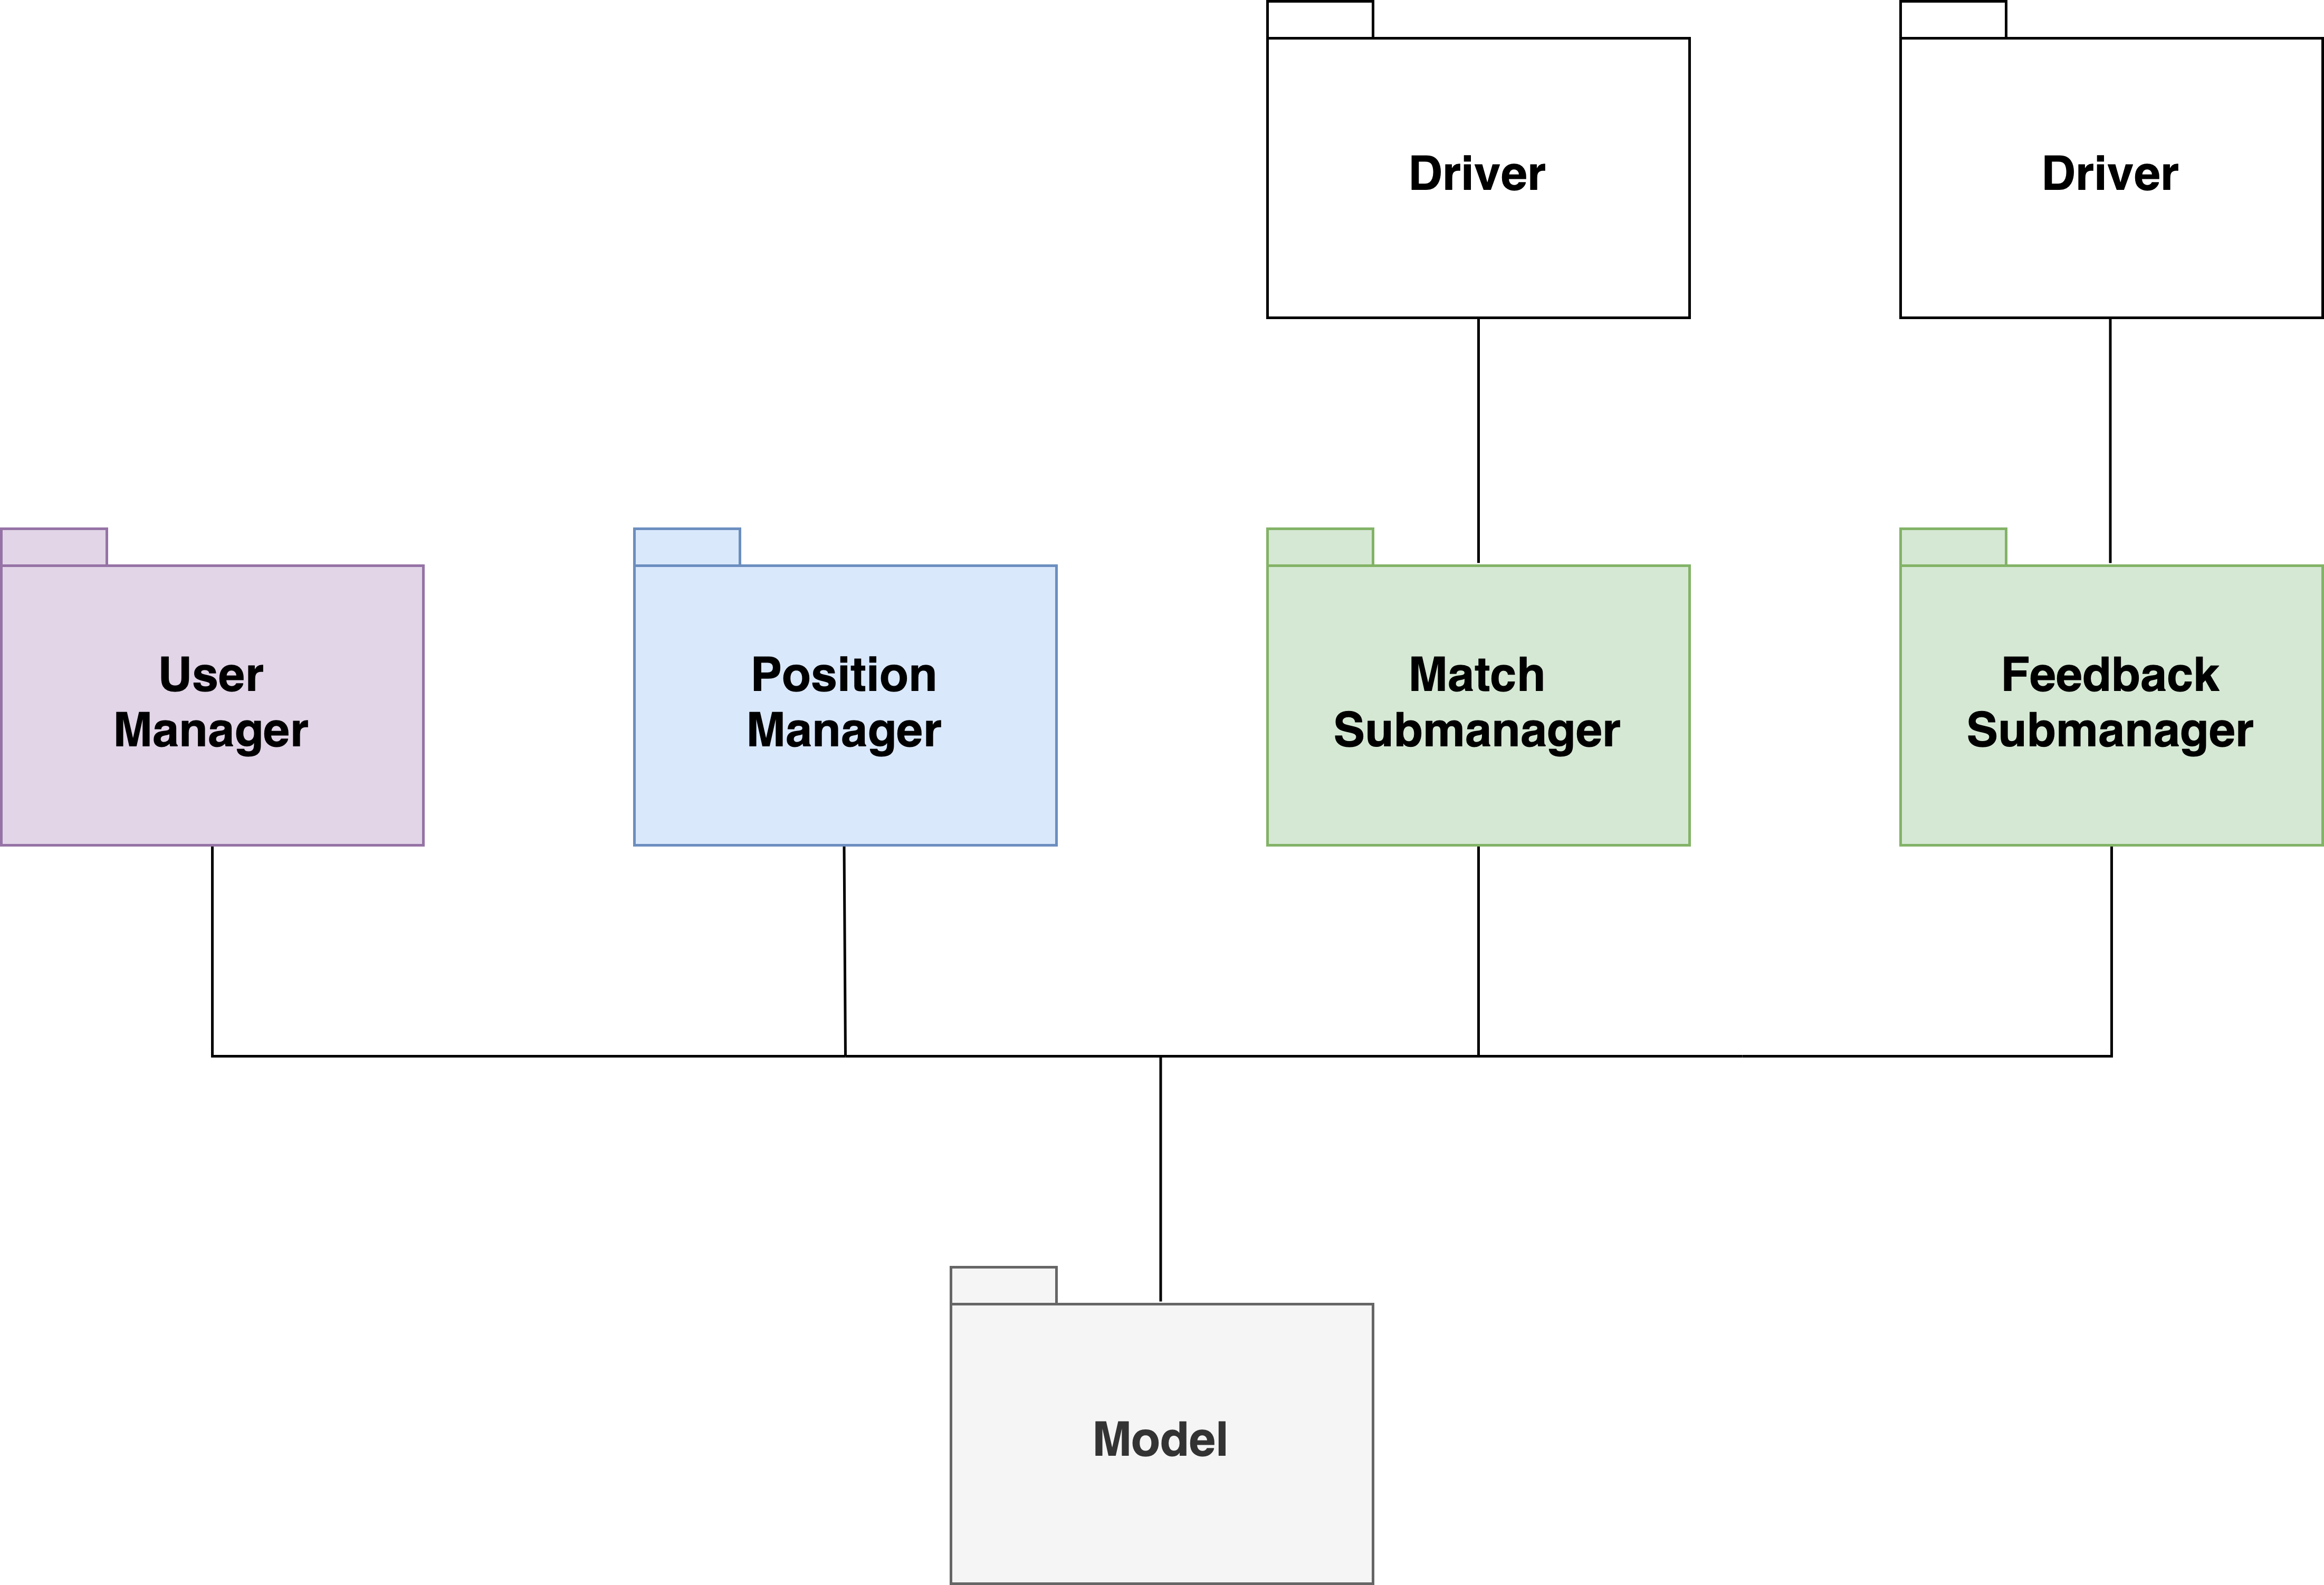
\includegraphics[width=13cm]{images/implementation-diagrams/step-6.png}
    \caption{Implementation step 6}
\end{figure}

\newpage
Step seven applies the same pattern to the selection application submanager.

\begin{figure}[h]
    \centering
    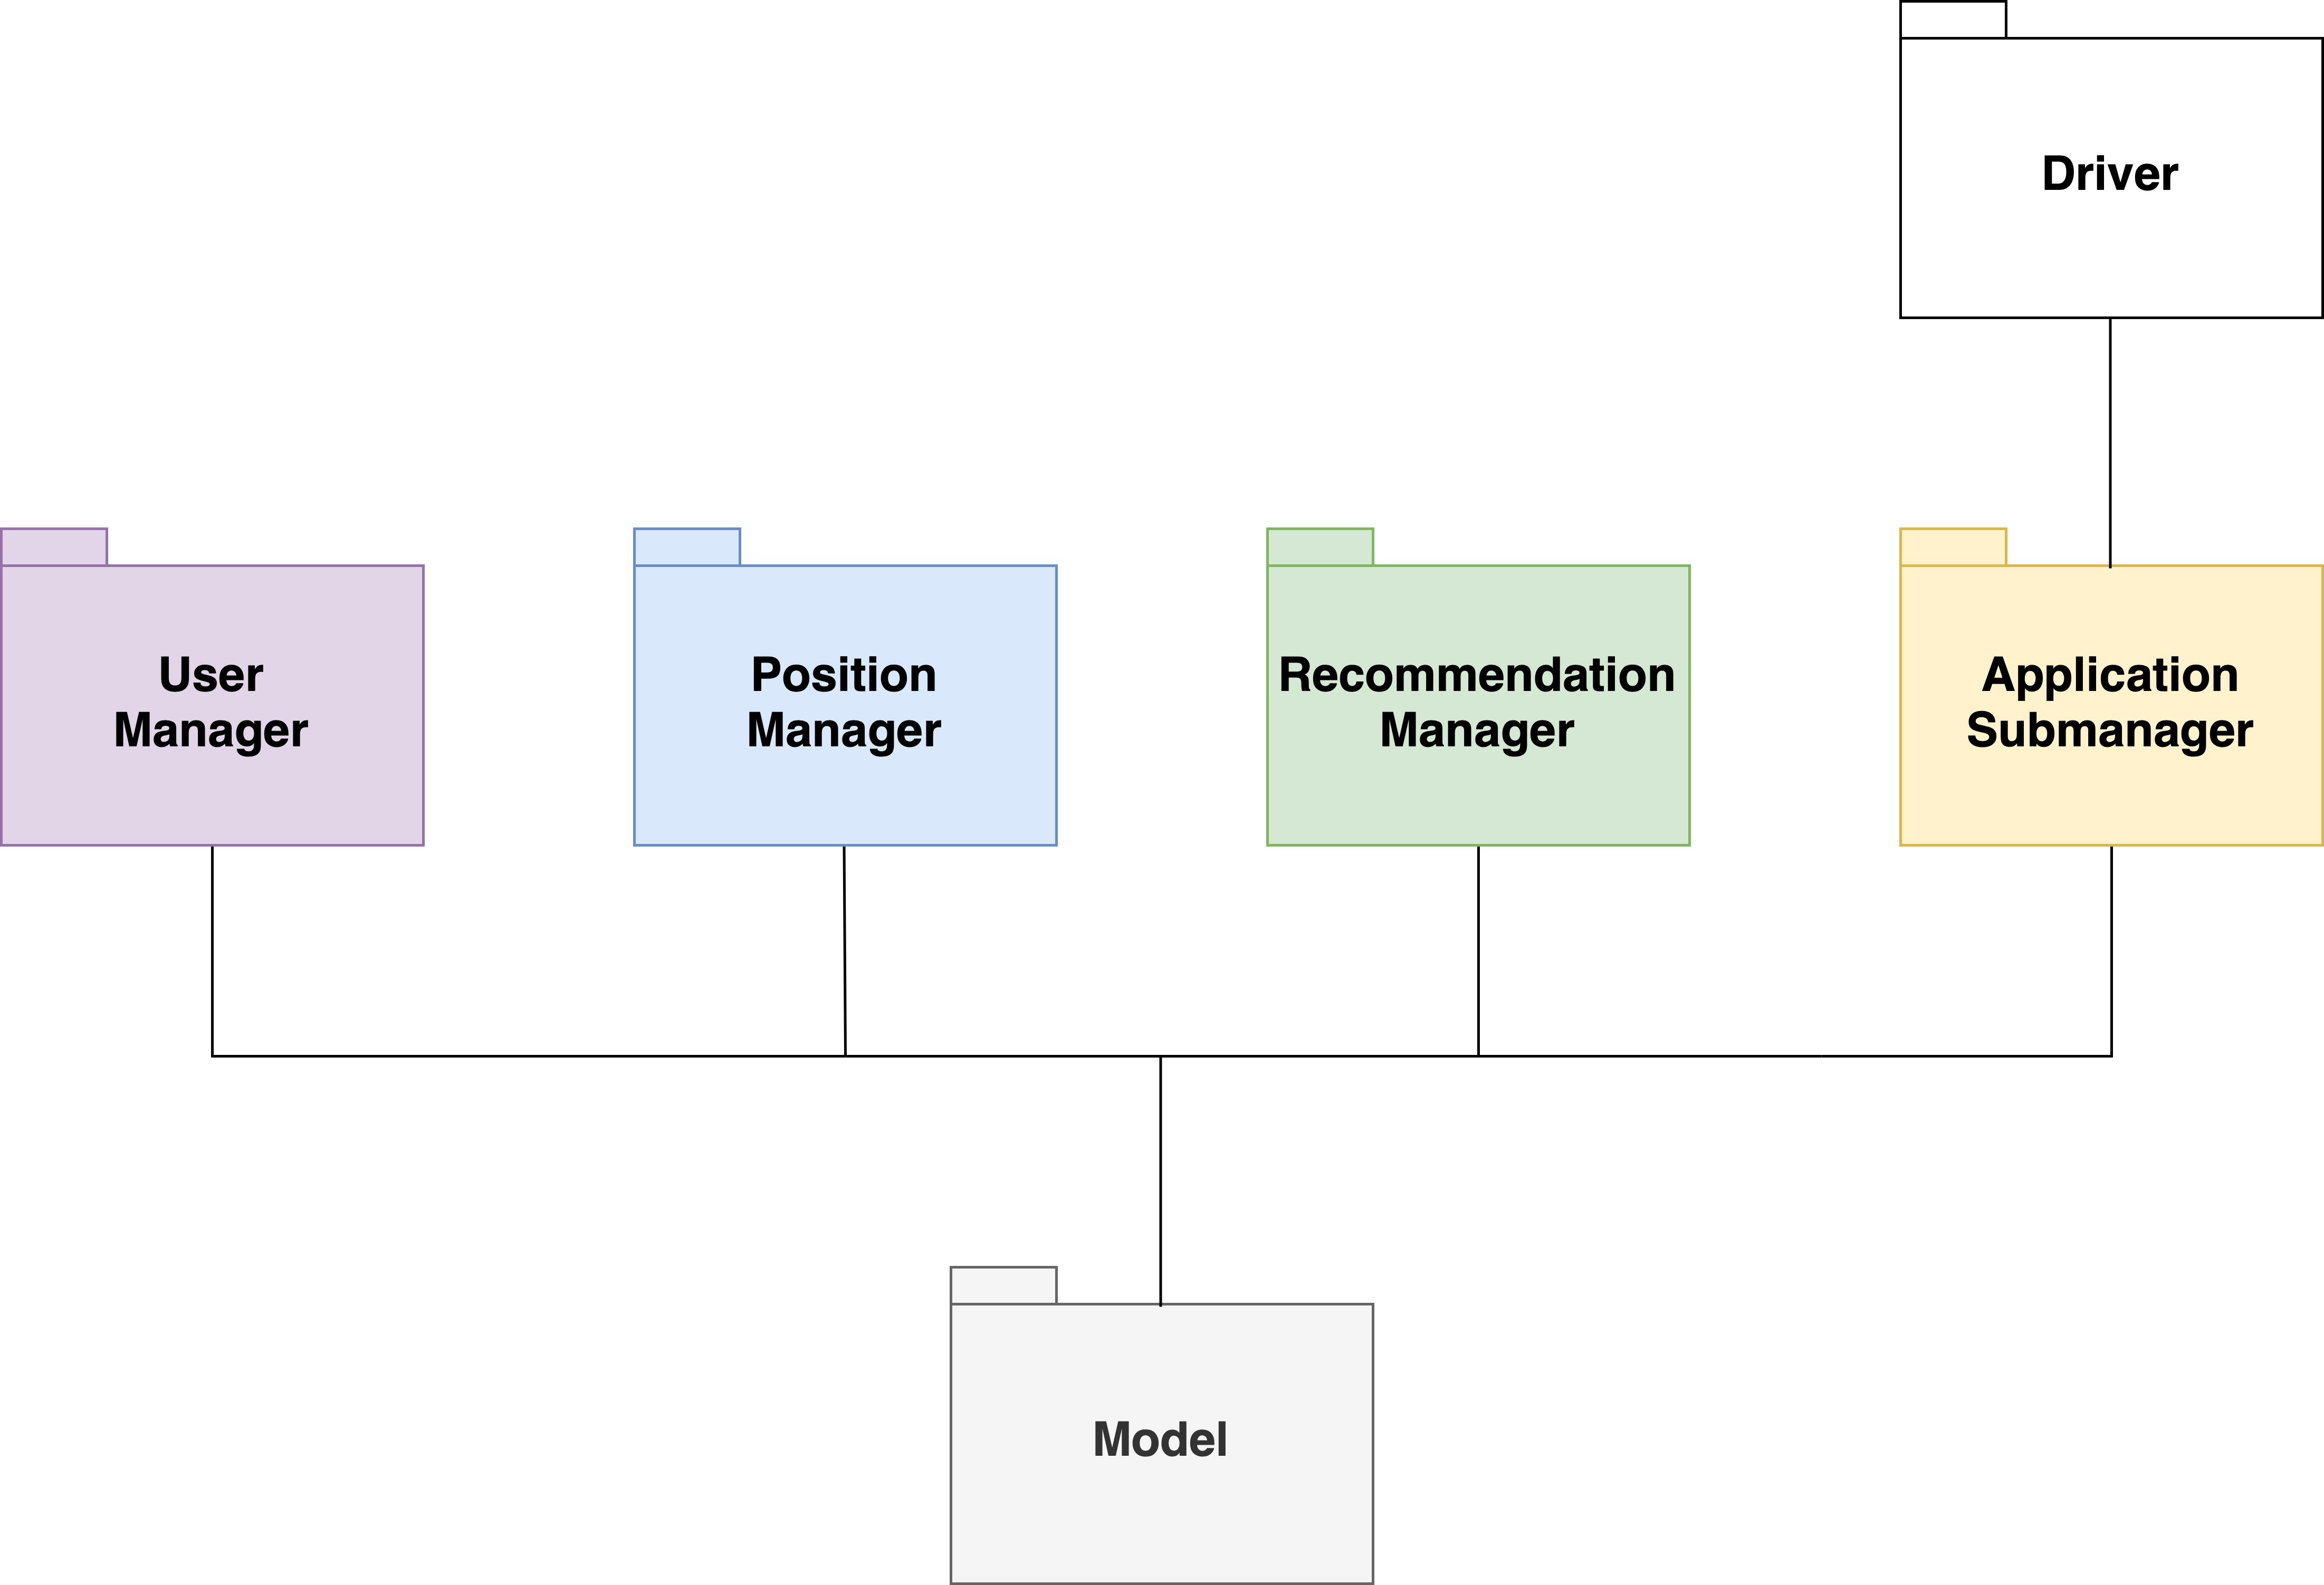
\includegraphics[width=13cm]{images/implementation-diagrams/step-7.png}
    \caption{Implementation step 7}
\end{figure}

\newpage
The selection interview and questionnaire submanagers are integrated in the eighth step.

\begin{figure}[h]
    \centering
    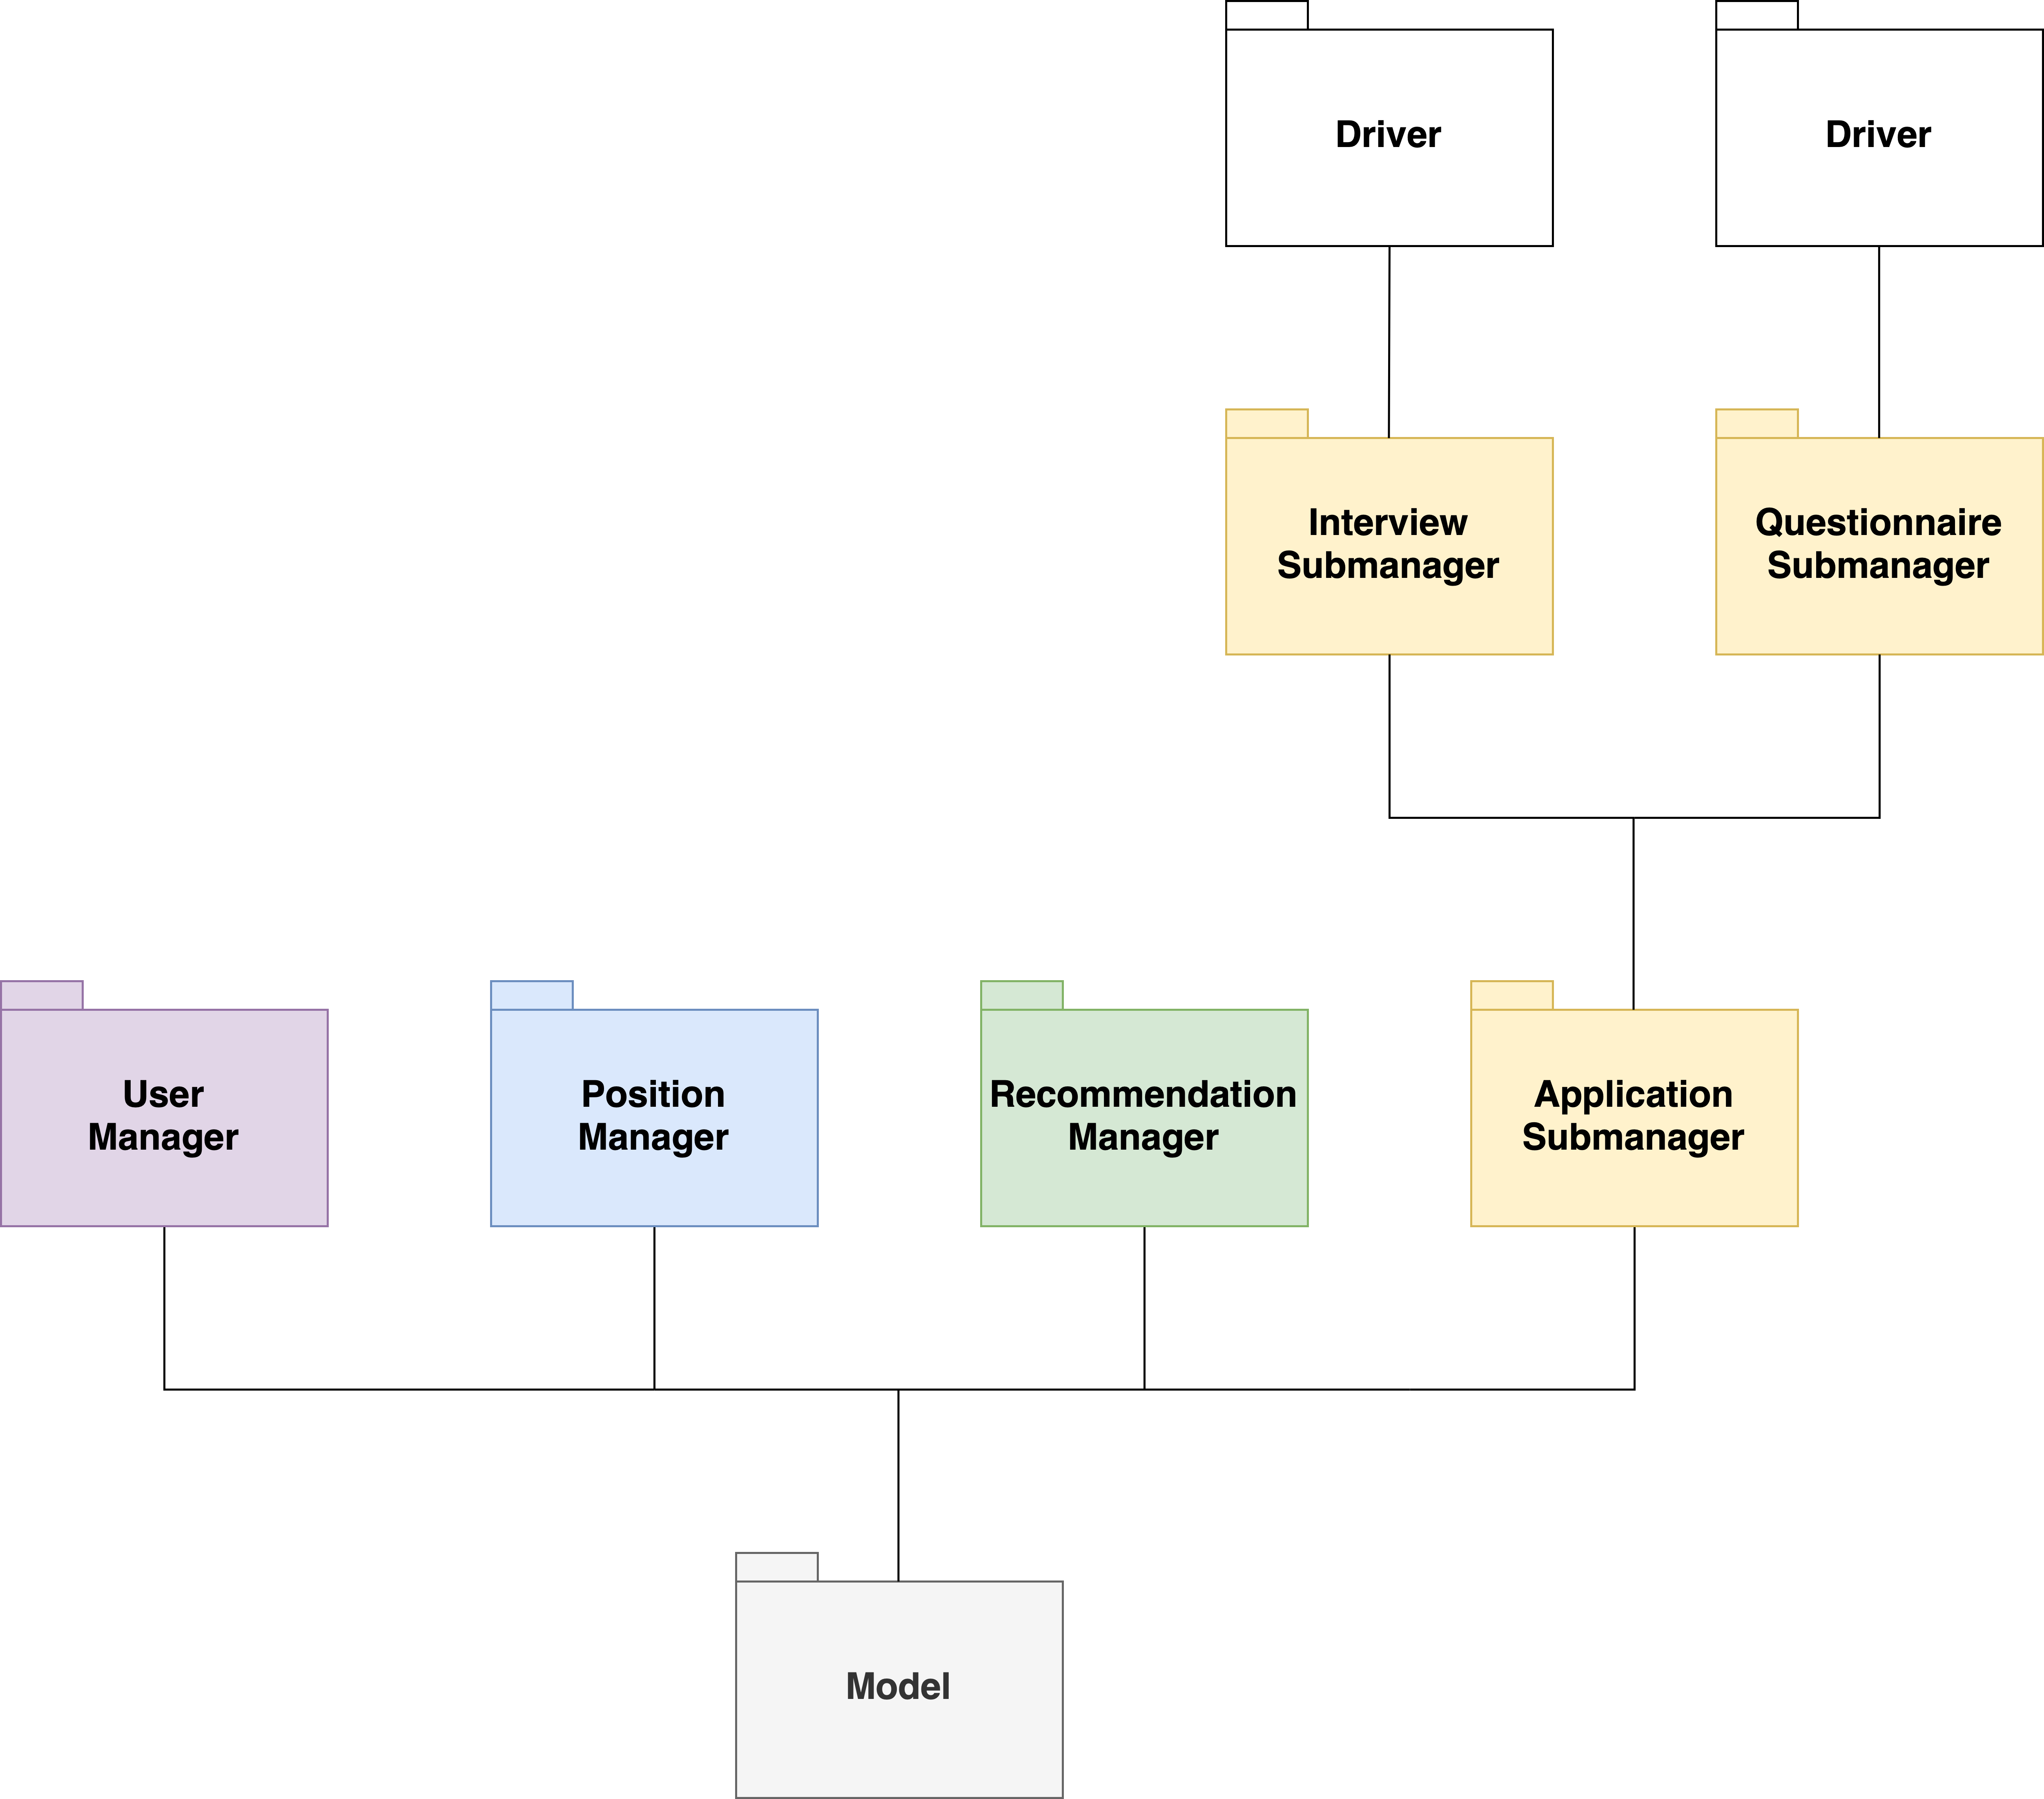
\includegraphics[width=14.5cm]{images/implementation-diagrams/step-8.png}
    \caption{Implementation step 8}
\end{figure}

\newpage
The development proceeds to step nine with the application submanagers.

\begin{figure}[h]
    \centering
    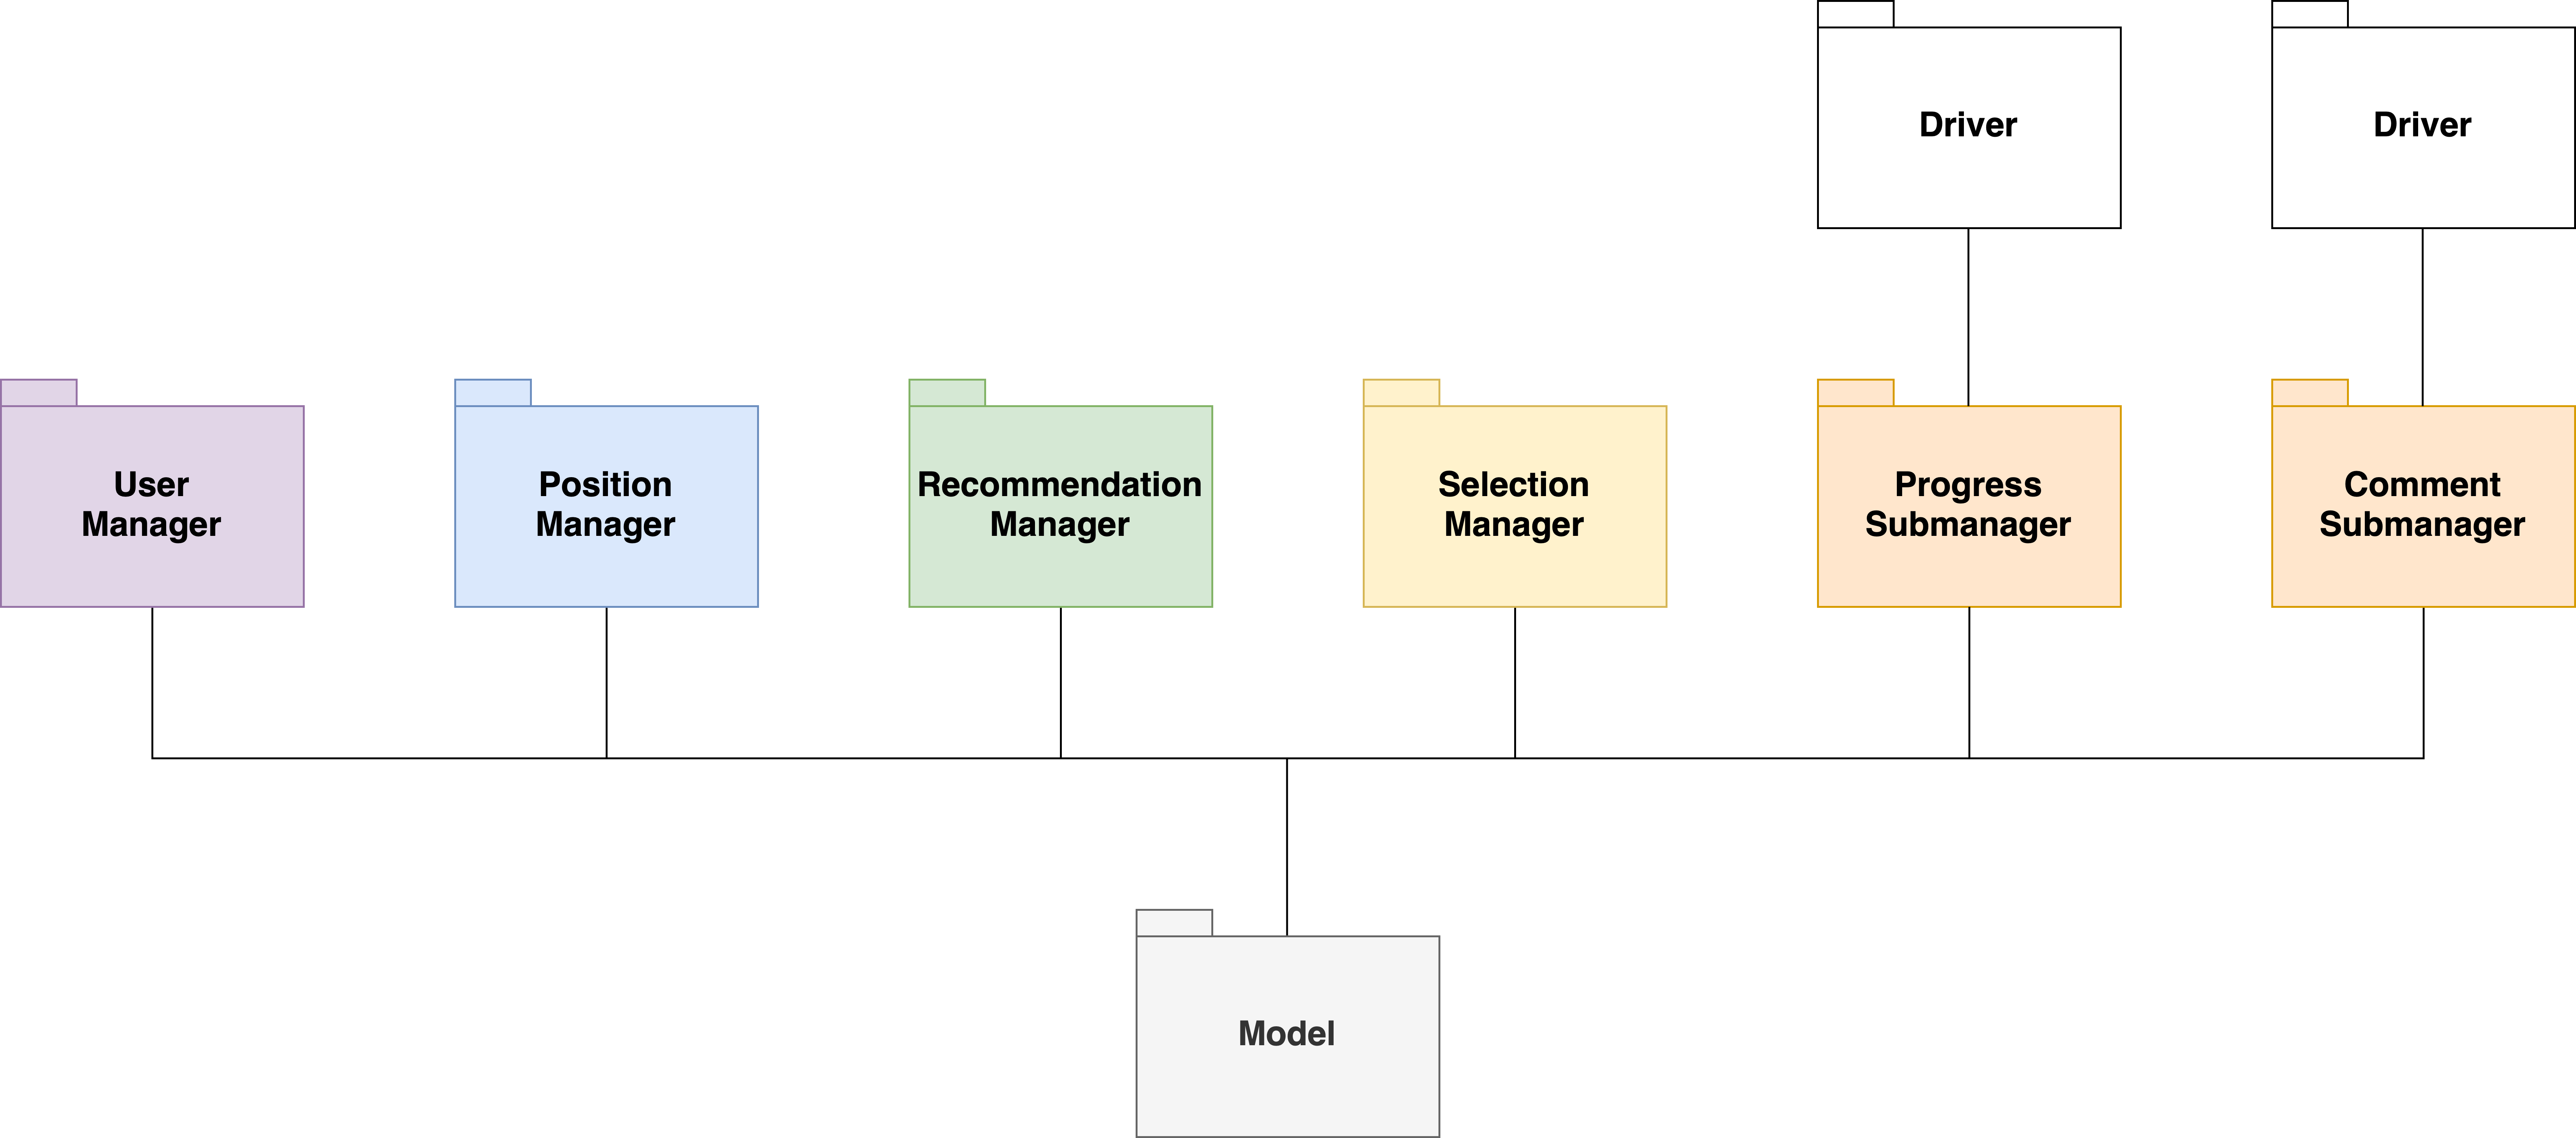
\includegraphics[width=16cm]{images/implementation-diagrams/step-9.png}
    \caption{Implementation step 9}
\end{figure}

\newpage
Step ten applies the same pattern to the notification submanagers.

\begin{figure}[h]
    \centering
    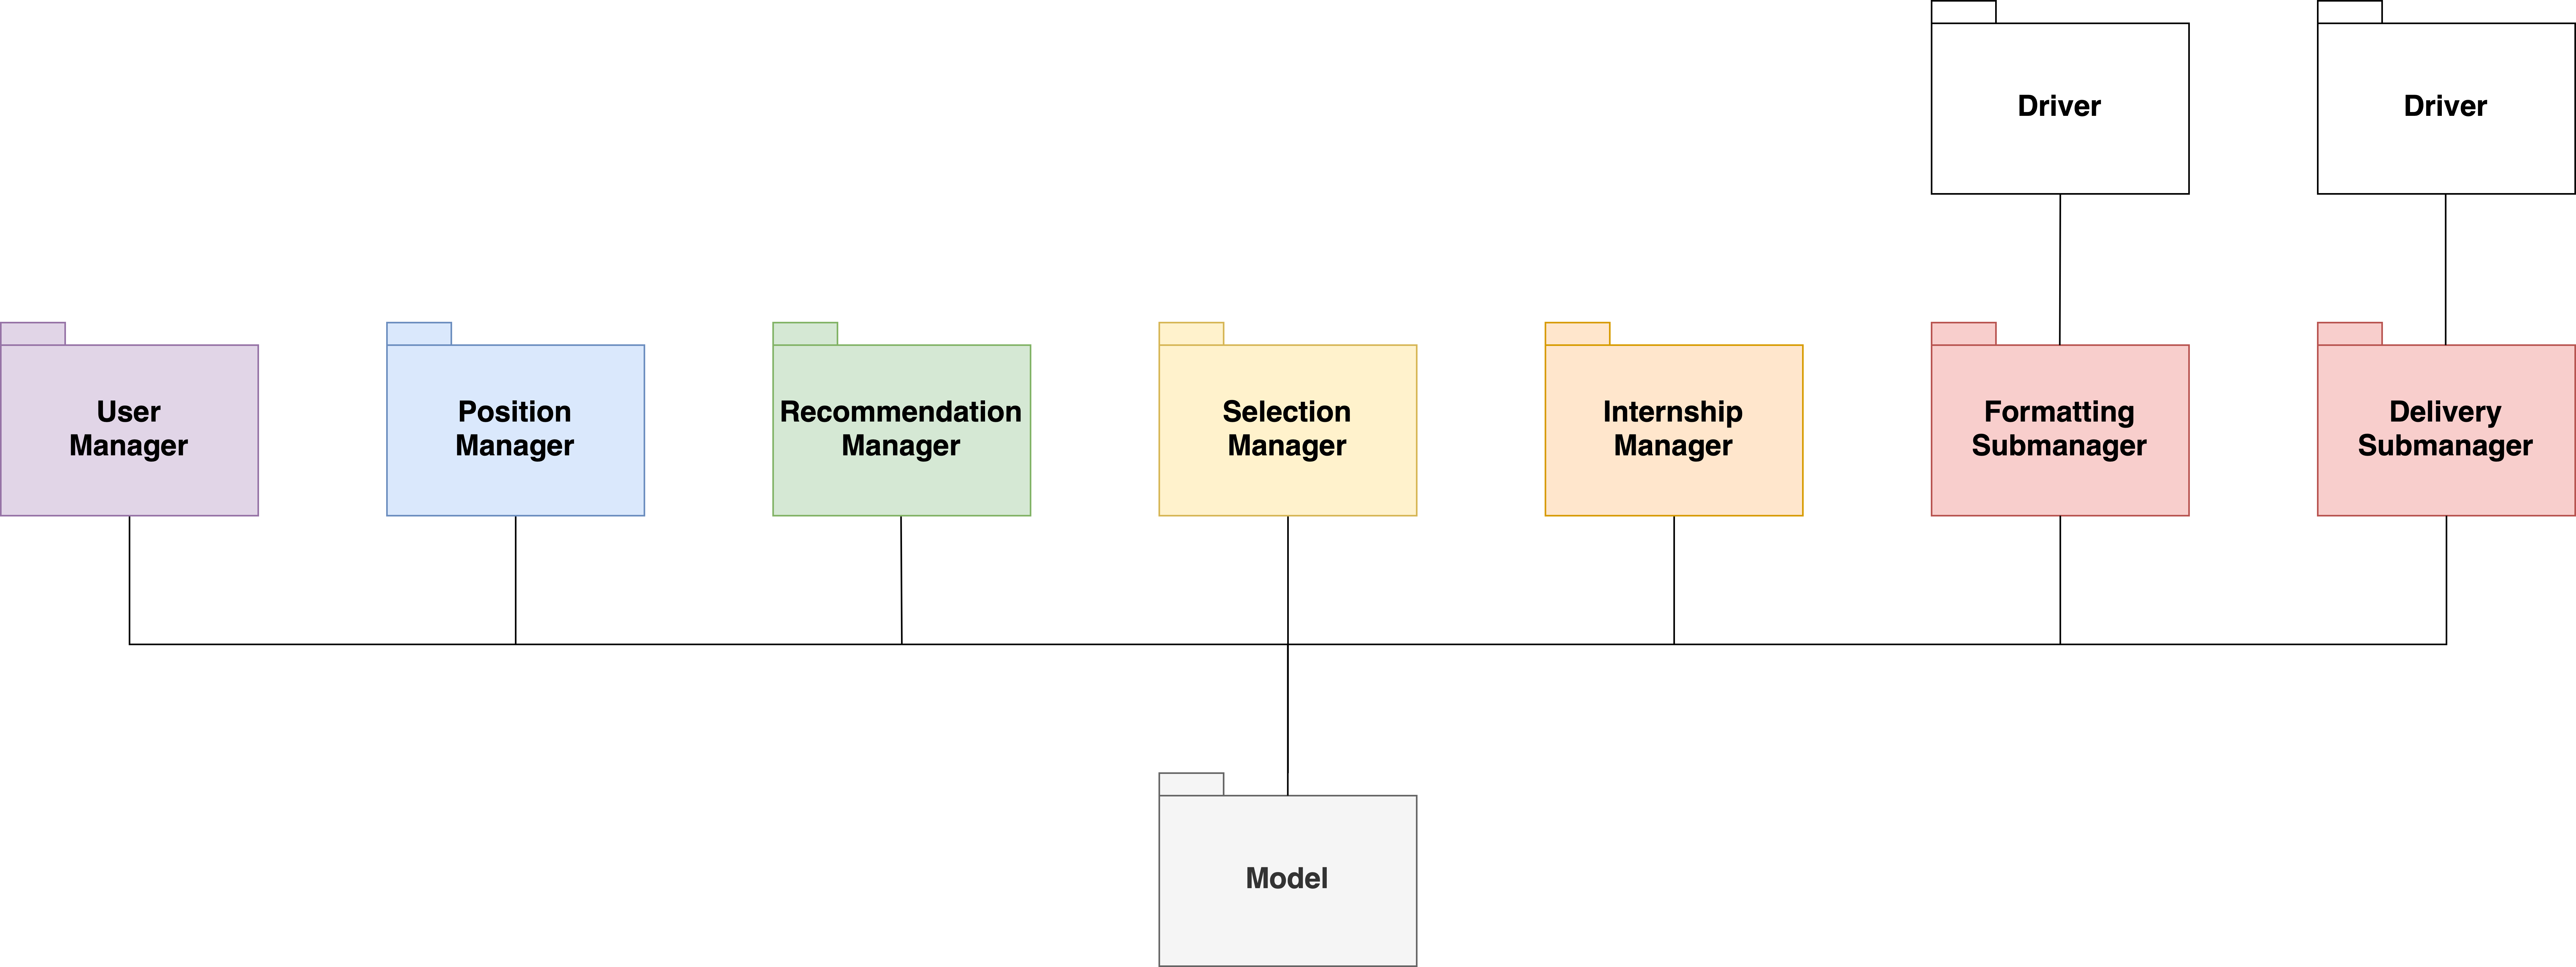
\includegraphics[width=16cm]{images/implementation-diagrams/step-10.png}
    \caption{Implementation step 10}
\end{figure}

\newpage
Note that the notification manager supports all implemented managers.

\begin{figure}[h]
    \centering
    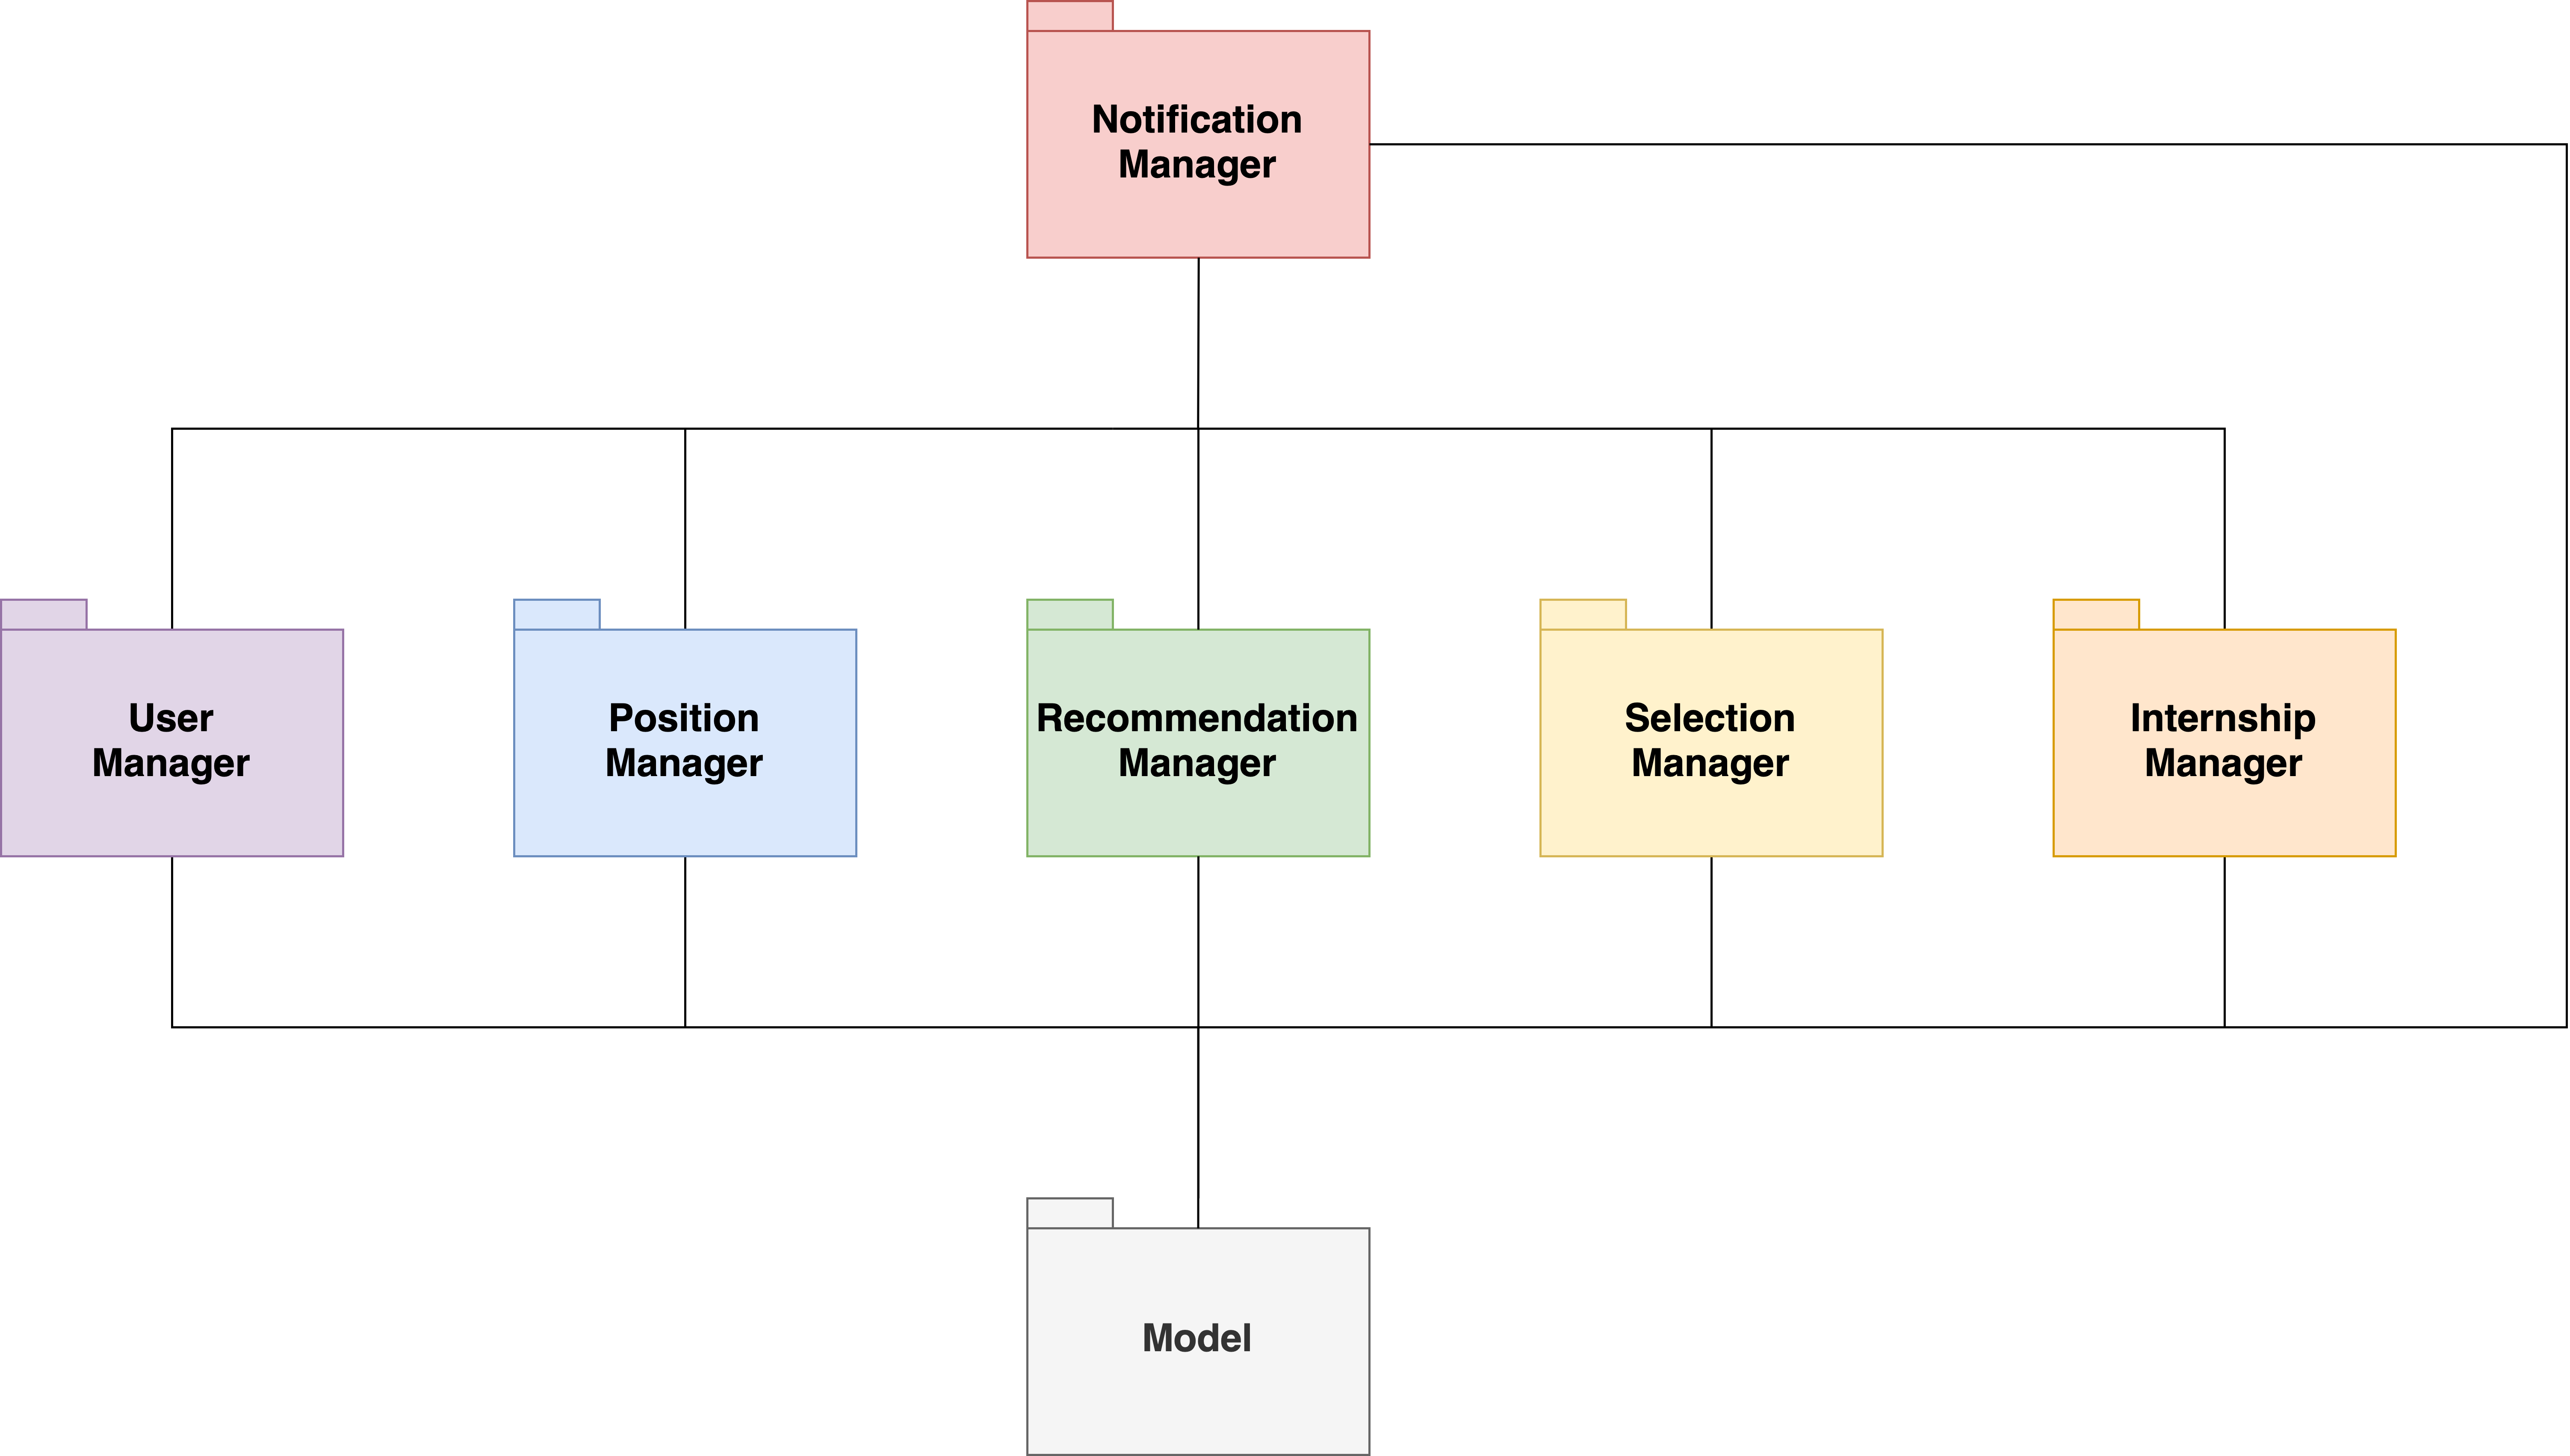
\includegraphics[width=16cm]{images/implementation-diagrams/step-11.png}
    \caption{Implementation step 11}
\end{figure}
